\section{Antitrust Enforcement and Leniency}\label{sec:12-enforcement}

The models of the previous sections treat collusion as a problem that firms solve among themselves. Competition law
adds a third party that can detect a cartel and punish it. This section asks how enforcement enters the incentive
constraints of a cartel. \Cref{sec:12-legal} describes the legal instruments. \Cref{sec:12-fines} adds fines to a
collude-or-compete supergame. \Cref{sec:12-chenrey} studies leniency programs in the model of \citet{ChenRey2013},
and \cref{sec:12-kaplow} discusses the critique by \citet{Kaplow2013} of the legal requirement of an agreement.

In this section $F$ denotes a fine. It is neither a fixed cost nor a distribution function. Page, equation and
proposition numbers for \citet{ChenRey2013} refer to their working-paper version of January 2012. We change the
paper's notation in two places. The detection probability $\rho$ becomes $\varrho$, because $\rho$ is pass-through
elsewhere in the book. The amnesty rate $q$ becomes $\ell$, because $q$ is a quantity.

\subsection{The legal framework}\label{sec:12-legal}

\Cref{sec:12-law} introduced the prohibitions of Section~1 of the Sherman Act and of Article~101, and noted that
individuals are jailed for cartel conduct every year. Here we describe the sanctions and the leniency programs that
enforce them. In the United States the Antitrust Division of the Department of Justice prosecutes price fixing as a
crime, against firms and against the executives involved. Fines per case have risen steeply since the early 1980s (\cref{sec:12-eu-facts}). The vitamin cartels of the 1990s show the scale. Roche paid a criminal fine of 500 million dollars
in the United States and BASF one of 225 million dollars. Purchasers recovered billions of dollars in damages through
civil litigation, and several executives of the major producers served time in prison
\citep[pp.~1--2]{MarshallMarx2012}. Private suits under the Sherman Act carry treble damages. Section~5 of the Federal
Trade Commission Act, by contrast, allows no private suits, treble damages or criminal penalties
\citep[p.~60, note~21]{Kaplow2013}. Kaplow regards the threat of imprisonment and fines on individuals as a
useful supplement to corporate fines, given agency problems within firms (p.~12). \citet[footnote~8]{ChenRey2013}
give 100 million dollars as the statutory maximum for a corporate fine in the United States. The vitamin fines show
that this maximum is not a hard ceiling. U.S. law also allows an alternative fine based on the gain from the offense
or on the loss it caused. A convicted organization may be fined up to the greater of twice the gross gain and twice
the gross loss to others \citep[\S~3571(c)(2) and (d)]{USCode2024}. The alternative does not apply when imposing it would
unduly complicate or prolong the sentencing process.
In the European Union the Commission imposes administrative fines of up to 10 percent of a firm's turnover
\citep[footnote~8]{ChenRey2013}. Under the Commission's 2006 guidelines, the fine starts from an amount based on the
value of the sales affected by the cartel and on the number of years of infringement. The Commission then adjusts it
for the circumstances of the case \citep[footnote~8]{ChenRey2013}. \Cref{tab:12-eu-fines} lists the largest fines
imposed so far.

Cartels hide their agreements, so the hardest part of enforcement is proving that firms colluded. Leniency programs,
also called whistleblower programs, address this problem by rewarding a member that reports the cartel. The United
States adopted a corporate leniency program in 1978. Its 1993 revision introduced two
rules \citep[p.~1]{ChenRey2013}. The \emph{first-informant rule} makes amnesty automatic for the first firm that
reports before an investigation has begun and meets the policy's conditions, and only that firm qualifies. The
\emph{post-investigation amnesty rule} lets the first firm to come forward after an investigation has started qualify
under further conditions. Among them, the Antitrust Division of the Department of Justice must not yet have evidence
likely to yield a sustainable conviction. \citet[p.~50, footnote~21]{LevensteinSuslow2006} attribute the surge in U.S. prosecutions of
international cartels in the 1990s primarily to this revision. \citet{Miller2009} finds that the revision raised
cartel discoveries by 60 percent, as \cref{sec:12-eu-facts} describes. The European Commission adopted a program in
1996 and revised it in 2002 \citep[footnote~1]{ChenRey2013}. Under its 1996 notice, the EU program reduced fines by 75
to 100 percent for a report made before an investigation and by 50 to 75 percent once one was under way
\citep[footnote~6 and p.~29]{ChenRey2013}. The second tier applied only while the investigation had not yet found
sufficient grounds for proceedings (\cref{sec:13-institutions}). The Commission's current framework is its 2006 Notice
on Immunity from Fines and Reduction of Fines in Cartel Cases. It grants conditional full immunity to the first
qualifying firm. Later firms whose evidence adds significant value receive reductions of 30 to 50, 20 to 30 and up to
20 percent, in order. Programs differ elsewhere. South
Korea can pay monetary rewards to individual informants, and Greece never grants amnesty to repeat offenders
\citep[footnote~1 and p.~14]{ChenRey2013}.

Many recent prosecutions began with a report from inside or near the cartel. The U.S. investigation of the graphite
electrodes cartel started with a complaint by a steel firm, a customer of the cartel
\citep[p.~62]{LevensteinSuslow2006}. The stamp-auction ring studied by \citet{Asker2010} came to light after a dealer
outside the ring alerted the authorities. Asker also suggests that strong members kept weak ones inside the ring
because an expelled member could report it and seek leniency (\cref{sec:13-asker}). Leniency therefore shapes how a
cartel is organized as well as whether it survives. \Cref{sec:13-institutions} describes how the cartels studied in
\cref{ch:collusion-evidence} came to light and what this implies for the selection of observed cartels.

Enforcement raises three economic questions. How do fines and leniency change the incentive constraints of a
cartel? Which leniency rate deters collusion in the largest set of industries? Should leniency continue after an
investigation opens, extend to more than one informant, or extend to repeat offenders? The rest of this section
answers them with repeated-game models.

\subsection{Fines in the repeated game}\label{sec:12-fines}

We embed enforcement in the simplest collusion game, following \citet[Section~2]{ChenRey2013}. We state the model
for $N$ firms because it costs nothing, and we specialize to the duopoly that Chen and Rey study.

\casehead{The stage game}
In each period, $N$ identical firms choose whether to collude or to compete. If all collude, each earns a gross profit
$B > 0$, the \emph{stake} of collusion. If one firm deviates while the others collude, the deviator earns $NB$ and the
others earn zero. If firms compete, each earns zero. The Bertrand supergame of \cref{prop:12-bertrand} has this form.
With homogeneous goods and constant marginal cost, collusion at the monopoly price gives each firm
$B = \frac{\pi^m}{N}$. A deviator slightly undercuts and captures nearly the whole monopoly profit $\pi^m = NB$.
Competition gives zero profit, which is both the static Nash payoff and the minmax payoff. Without enforcement, grim
trigger sustains collusion if and only if
\begin{equation*}
\frac{B}{1-\delta} \ge NB \iff \delta \ge 1 - \frac{1}{N}.
\end{equation*}
The industries of the economy share the discount factor $\delta$ and differ in the stake $B$. A larger $B$ makes
collusion more profitable and also raises the one-period gain from a deviation.

\begin{assumption}[Enforcement without leniency]\label{asm:12-enforcement}
\leavevmode
\begin{enumerate}[label=(\roman*)]
\item In each period, collusion generates evidence if and only if all firms agree to collude at the start of the
period. The evidence lasts one period, so a cartel cannot be prosecuted for past periods.
\item In each period with evidence, the authority finds it with probability $\varrho \in (0,1)$, independently across
periods. Each firm then pays the fine $F > 0$.
\item The discount factor satisfies $\delta > \frac{N-1}{N}$, so that collusion is a concern absent enforcement.
\item A deviation from the collusive agreement is followed by competition forever.
\end{enumerate}
\end{assumption}

The timing within a period has three stages. At stage~0 each firm decides whether to enter a collusive agreement. If
any firm refuses, the firms compete and the period ends. At stage~1 each firm colludes or deviates in the product
market, and rivals observe the choice only at the end of the period. At stage~2 firms may report the evidence to the
authority. Without a leniency program a report only exposes the reporter, so nobody reports.

\begin{definition}\label{def:12-deterrence}
The \emph{deterrence threshold} of an enforcement policy is the smallest stake $B$ at which collusion is a subgame
perfect equilibrium outcome. The policy deters collusion in every industry whose stake lies below the threshold.
\end{definition}

Because industries differ only in $B$, a policy with a higher threshold deters collusion in a superset of
industries. Maximizing the deterrence threshold is therefore optimal whatever the distribution of stakes across
industries. This is the objective of the authority in \citet{ChenRey2013}.

\begin{proposition}[Collusion with fines]\label{prop:12-fines}
Under \cref{asm:12-enforcement}, \emph{normal collusion} (collude in every period, never report, compete forever after
a deviation) is a subgame perfect equilibrium if and only if
\begin{equation}\label{eq:12-fines-threshold}
B \ge \underline B \equiv \frac{\delta\varrho F}{N\delta - (N-1)}.
\end{equation}
For $N = 2$ the threshold is $\underline B = \frac{\delta\varrho F}{2\delta - 1}$, equation~(1) of
\citet{ChenRey2013}. The threshold $\underline B$ rises with $\varrho$, with $F$ and with $N$, and falls with
$\delta$.
\end{proposition}

\begin{proof}
On the collusive path each firm earns $B$ and pays the fine $F$ with probability $\varrho$ in every period. The value
of normal collusion is
\begin{equation}\label{eq:12-fines-VN}
V_N = \sum_{t=0}^{\infty}\delta^t (B - \varrho F) = \frac{B - \varrho F}{1-\delta}.
\end{equation}
The punishment phase repeats the static Nash equilibrium, so it is subgame perfect (\cref{prop:12-static-repeat}). By
the one-shot deviation principle (\cref{prop:12-osdp}), it remains to check one-period deviations on the collusive
path. Consider first a deviation at stage~1. The deviator earns $NB$. All firms agreed at stage~0, so evidence exists
and the deviator still pays $F$ with probability $\varrho$. From the next period on it earns zero. The deviation is
unprofitable if and only if
\begin{align*}
\frac{B - \varrho F}{1-\delta} &\ge NB - \varrho F\\
B - \varrho F &\ge (1-\delta)NB - (1-\delta)\varrho F\\
B\,[1 - N(1-\delta)] &\ge \delta\varrho F.
\end{align*}
Part~(iii) of \cref{asm:12-enforcement} gives $1 - N(1-\delta) = N\delta - (N-1) > 0$. Dividing by it yields
\eqref{eq:12-fines-threshold}.

Consider next a refusal at stage~0. It yields zero in the current period and zero afterwards, so it is unprofitable
if and only if $V_N \ge 0$, that is, $B \ge \varrho F$. The threshold satisfies $\underline B \ge \varrho F$, because
\begin{equation*}
\frac{\delta}{N\delta - (N-1)} \ge 1 \iff (N-1)(1-\delta) \ge 0.
\end{equation*}
Hence every $B \ge \underline B$ also deters a refusal, and the stage-1 deviation is the binding one.

For the comparative statics, the numerator of $\underline B$ rises with $\varrho$ and $F$. The denominator falls with
$N$, because its derivative with respect to $N$ is $\delta - 1 < 0$. Finally,
\begin{equation*}
\frac{\partial \underline B}{\partial \delta}
= \varrho F\,\frac{[N\delta - (N-1)] - N\delta}{[N\delta - (N-1)]^2}
= -\frac{(N-1)\varrho F}{[N\delta - (N-1)]^2} < 0. \qedhere
\end{equation*}
\end{proof}

The incentive constraint has a transparent form. Rearranging the third line of the proof gives
\begin{equation}\label{eq:12-fines-ic}
\frac{\delta}{1-\delta}\,(B - \varrho F) \ge (N-1)B.
\end{equation}
The left side is the discounted value of future collusion net of expected fines. The right side is the one-period
gain from a deviation. The expected fine of the current period does not appear, because the deviator pays it as
well. Fines deter collusion only by lowering the value of future collusion. Enforcement thus works like a fall in
the discount factor. It deters collusion in industries with small stakes and leaves large-stake industries
untouched.

\begin{remark}[Maximal fines and fines proportional to the stake]\label{rem:12-fine-caps}
Deterrence depends on the expected fine $\varrho F$. Raising $F$ is cheap, while raising $\varrho$ requires
investigations. The economics of optimal enforcement \citep{Becker1968,PolinskyShavell2000} therefore recommends
setting the fine at its maximum, and \citet{ChenRey2013} interpret $F$ as the maximal fine. In practice fines are
capped by law, as described in \cref{sec:12-legal}. The model takes $F$ to be independent of $B$. Suppose instead that
the fine is proportional to the stake, $F = \phi B$, as the EU guidelines suggest by basing fines on affected sales.
Then \eqref{eq:12-fines-threshold} becomes
\begin{equation*}
N\delta - (N-1) \ge \delta\varrho\phi,
\end{equation*}
which does not depend on $B$. Enforcement then deters collusion either in every industry or in none. Heterogeneity in
stakes matters for policy design only because fines do not scale with the gains from collusion. Private damages
raise the expected sanction further. \citet[p.~62, footnote~60]{LevensteinSuslow2006} note an argument that customers
may anticipate damages in their demand, so that only unanticipated damages deter.
\end{remark}

\subsection{Chen and Rey (2013): the design of leniency programs}\label{sec:12-chenrey}

\casehead{Question}
Leniency programs have two opposite effects. They destabilize collusion, because a member can cheat and report,
escaping part of the fine. They can also lower the expected fine of a cartel that has no intention of breaking up.
\citet[p.~349]{MottaPolo2003}, as quoted by \citet[p.~1]{ChenRey2013}, warn that reduced fines may have an ex ante
pro-collusive effect. \citet[p.~137]{Wils2008}, also quoted there, imagines cartel members that take turns applying for
leniency whenever a cartel is about to be detected. Earlier work mostly took the leniency rate as given.
\citet{ChenRey2013} ask which amnesty rate deters collusion in the largest set of industries. They also ask whether
leniency should continue after an investigation starts, whether it should be restricted to the first informant, and
whether repeat offenders should be excluded.

\casehead{Setting and model}
Chen and Rey study the duopoly version of \cref{asm:12-enforcement}, so $N = 2$ and a deviator earns $2B$. Absent
enforcement, collusion requires $\delta \ge \frac{1}{2}$, and they assume $\delta > \frac{1}{2}$. A leniency program
changes stage~2. If at least one firm reports, the cartel is detected for sure. The first informant pays the reduced
fine $(1-\ell)F$ and the other firm pays $F$. The parameter $\ell$ is the \emph{amnesty rate}. A value
$\ell \in [0,1]$ is a fine reduction, and $\ell > 1$ is a reward of $(\ell - 1)F$. If nobody reports, the authority
detects the cartel with probability $\varrho$, and both firms pay $F$. In this first version investigations are
secret, so firms do not know whether one is under way. The policy is stationary and treats all industries alike. The
paper contains no data. Its empirical content comes from laboratory evidence and from the policy facts of
\cref{sec:12-legal}.

Leniency enlarges the set of collusive strategies. Chen and Rey show that two of them matter
\citep[p.~10 and footnote~12]{ChenRey2013}.
\begin{itemize}
\item \emph{Normal collusion} (N). Firms collude in every period and never report. After a deviation they compete
forever.
\item \emph{Collude and report} (R). Firms collude in every period, and both report the evidence at stage~2 of every
period. Each is the first informant with probability $\frac{1}{2}$. After a product-market deviation they compete
forever.
\end{itemize}
They also argue that no other form of collusion is sustainable when these two are not. Symmetric strategies and
collusion in every period maximize the value of collusion, and randomizing between reporting and not reporting is
not sustainable when neither pure strategy is.

\casehead{Normal collusion under leniency}
Leniency adds a new deviation to normal collusion, ``cheat and report.''

\begin{lemma}\label{lem:12-cr-report}
Under normal collusion, a firm that deviates in the product market prefers to report at stage~2 if and only if
\begin{equation}\label{eq:12-cr-qlow}
\ell > \underline\ell \equiv 1 - \varrho.
\end{equation}
A firm that colludes and then reports is worse off than a firm that deviates and reports.
\end{lemma}

\begin{proof}
After a deviation the firms compete forever whether or not the deviator reports, so only the current fine matters. The
rival does not plan to report, so a reporting deviator is the first informant and pays $(1-\ell)F$. A silent deviator
pays $F$ with probability $\varrho$. Reporting is better if and only if $(1-\ell)F < \varrho F$, which is
\eqref{eq:12-cr-qlow}. A firm that colludes and reports earns $B$ instead of $2B$ in the current period, pays the same
fine, and faces the same competitive future, since its report breaks the agreement.
\end{proof}

When $\ell > \underline\ell$, the relevant deviation yields $2B - (1-\ell)F$, and normal collusion survives it if
and only if
\begin{align*}
\frac{B - \varrho F}{1-\delta} &\ge 2B - (1-\ell)F\\
B - \varrho F &\ge 2(1-\delta)B - (1-\delta)(1-\ell)F\\
(2\delta - 1)B &\ge [\varrho - (1-\delta)(1-\ell)]F.
\end{align*}
Hence normal collusion requires
\begin{equation}\label{eq:12-cr-BNr}
B \ge B_N^r(\ell) \equiv \frac{\varrho - (1-\delta)(1-\ell)}{2\delta - 1}\,F,
\end{equation}
which is equation~(2) of \citet{ChenRey2013}. The threshold rises linearly in $\ell$. Comparing it with
$\underline B = \frac{\delta\varrho F}{2\delta-1}$ gives
\begin{equation}\label{eq:12-cr-BNr-minus}
B_N^r(\ell) - \underline B = \frac{(1-\delta)(\ell - \underline\ell)}{2\delta - 1}\,F.
\end{equation}
Leniency makes normal collusion harder exactly when it induces deviators to report. Normal collusion is sustainable
if and only if
\begin{equation}\label{eq:12-cr-BN}
B \ge B_N(\ell) \equiv \max\{\underline B,\, B_N^r(\ell)\}.
\end{equation}

\casehead{Collude and report}
Under collude and report, each firm pays the reduced fine with probability $\frac{1}{2}$ and the full fine otherwise.
Its expected fine per period is $\frac{1}{2}(1-\ell)F + \frac{1}{2}F = (1 - \frac{\ell}{2})F$. The value of this
form of collusion is
\begin{equation}\label{eq:12-cr-VR}
V_R(\ell) = \frac{B - \left(1 - \frac{\ell}{2}\right)F}{1-\delta}.
\end{equation}
Reporting is self-enforcing. If the rival reports, a silent firm pays $F$, while a reporting firm pays
$(1 - \frac{\ell}{2})F < F$ in expectation, for any $\ell > 0$. A product-market deviator therefore still reports.
Chen and Rey assume that the two reports are not ranked by a race, so the deviator is the first informant with
probability $\frac{1}{2}$ \citep[footnote~11]{ChenRey2013}. The deviation yields $2B - (1 - \frac{\ell}{2})F$ and then
zero. Collude and report is sustainable if and only if
\begin{align*}
\frac{B - \left(1 - \frac{\ell}{2}\right)F}{1-\delta} &\ge 2B - \left(1 - \frac{\ell}{2}\right)F\\
B - \left(1 - \frac{\ell}{2}\right)F &\ge 2(1-\delta)B - (1-\delta)\left(1 - \frac{\ell}{2}\right)F\\
(2\delta - 1)B &\ge \delta\left(1 - \frac{\ell}{2}\right)F.
\end{align*}
Hence collude and report requires
\begin{equation}\label{eq:12-cr-BR}
B \ge B_R(\ell) \equiv \frac{\delta\left(1 - \frac{\ell}{2}\right)}{2\delta - 1}\,F,
\end{equation}
which is equation~(3) of \citet{ChenRey2013}. This threshold falls in $\ell$. More generous leniency lowers the
expected fine of a reporting cartel and makes it more robust. It is more robust than normal collusion without leniency
when $B_R(\ell) < \underline B$, that is, when $1 - \frac{\ell}{2} < \varrho$, or
\begin{equation}\label{eq:12-cr-qbar}
\ell > \bar\ell \equiv 2(1 - \varrho).
\end{equation}
We call such rates \emph{excessive leniency}. The threshold is twice the rate at which deviators start to report,
$\bar\ell = 2\underline\ell$.

\casehead{The optimal amnesty rate}
Some form of collusion is sustainable in an industry if and only if $B \ge \min\{B_N(\ell), B_R(\ell)\}$. The
authority therefore chooses $\ell$ to maximize the deterrence threshold
\begin{equation}\label{eq:12-cr-objective}
B(\ell) \equiv \min\{B_N(\ell),\, B_R(\ell)\}.
\end{equation}

\begin{proposition}[Optimal leniency, \citealp{ChenRey2013}, Proposition~1]\label{prop:12-chen-rey}
Let $\frac{1}{2} < \delta < 1$ and $0 < \varrho < 1$.
\begin{enumerate}[label=(\alph*)]
\item The deterrence threshold $B(\ell)$ has a unique maximizer,
\begin{equation}\label{eq:12-cr-qhat}
\hat\ell(\varrho) = \frac{1 - \varrho}{1 - \frac{\delta}{2}},
\end{equation}
which satisfies $\underline\ell < \hat\ell < \bar\ell$. It solves $B_N^r(\hat\ell) = B_R(\hat\ell)$.
\item The maximal deterrence threshold is
\begin{equation}\label{eq:12-cr-Bhat}
\hat B(\varrho) = \frac{\delta(1 - \delta + \varrho)}{(2\delta - 1)(2 - \delta)}\,F > \underline B.
\end{equation}
\item The optimal rate $\hat\ell$ falls as $\varrho$ rises, and it exceeds 1, so that the first informant receives a
reward, if and only if $\varrho < \frac{\delta}{2}$. The threshold $\hat B$ rises with $\varrho$.
\item In industries with $B \ge \hat B$, both forms of collusion are sustainable at $\ell = \hat\ell$, and normal
collusion is more valuable:
\begin{equation}\label{eq:12-cr-VN-VR}
V_N - V_R(\hat\ell) = \frac{1 - \varrho}{2 - \delta}\,F > 0.
\end{equation}
\end{enumerate}
Equations \eqref{eq:12-cr-qhat} and \eqref{eq:12-cr-Bhat} are equations~(4) and~(5) of \citet{ChenRey2013}.
\end{proposition}

\begin{proof}
We first describe the two functions. By \eqref{eq:12-cr-BNr-minus}, $B_N(\ell) = \underline B$ for
$\ell \le \underline\ell$, and $B_N(\ell) = B_N^r(\ell)$ is strictly increasing for $\ell \ge \underline\ell$. The
function $B_R(\ell)$ is strictly decreasing.

\emph{Step 1 (no leniency below $\underline\ell$ helps).} At $\ell = \underline\ell = 1 - \varrho$ we have
$1 - \frac{\underline\ell}{2} = \frac{1+\varrho}{2}$, so
\begin{equation*}
B_R(\underline\ell) = \frac{\delta(1+\varrho)}{2(2\delta - 1)}\,F > \frac{\delta\varrho}{2\delta - 1}\,F = \underline B,
\end{equation*}
because $\frac{1+\varrho}{2} > \varrho$ when $\varrho < 1$. Since $B_R$ is decreasing, $B_R(\ell) > \underline B$ for
all $\ell \le \underline\ell$. Hence $B(\ell) = \underline B$ on $[0, \underline\ell]$.

\emph{Step 2 (excessive leniency hurts).} At $\ell = \bar\ell$ we have $1 - \frac{\bar\ell}{2} = \varrho$, so
$B_R(\bar\ell) = \underline B$. For $\ell \ge \bar\ell$, $B(\ell) \le B_R(\ell) \le \underline B$.

\emph{Step 3 (the crossing).} On $(\underline\ell, \bar\ell)$, $B_N = B_N^r$ is increasing and $B_R$ is decreasing. At
$\underline\ell$, $B_N^r = \underline B < B_R$. At $\bar\ell$, $B_N^r > \underline B = B_R$. The two lines cross at a
unique $\hat\ell \in (\underline\ell, \bar\ell)$. To the left of $\hat\ell$ the minimum is $B_N^r$, which rises. To
the right it is $B_R$, which falls. So $\hat\ell$ maximizes $B(\ell)$, and $\hat B = B_N^r(\hat\ell) >
B_N^r(\underline\ell) = \underline B$.

\emph{Step 4 (closed forms).} Setting $B_N^r(\ell) = B_R(\ell)$ and cancelling $\frac{F}{2\delta-1}$ gives
\begin{align*}
\varrho - (1-\delta)(1-\ell) &= \delta\left(1 - \frac{\ell}{2}\right)\\
\ell\left[(1-\delta) + \frac{\delta}{2}\right] &= \delta + (1-\delta) - \varrho\\
\ell\left(1 - \frac{\delta}{2}\right) &= 1 - \varrho,
\end{align*}
which is \eqref{eq:12-cr-qhat}. Substituting into $B_R$,
\begin{equation*}
1 - \frac{\hat\ell}{2} = 1 - \frac{1-\varrho}{2-\delta} = \frac{1 - \delta + \varrho}{2 - \delta},
\qquad\text{so}\qquad
\hat B = \frac{\delta}{2\delta - 1}\cdot\frac{1 - \delta + \varrho}{2 - \delta}\,F,
\end{equation*}
which is \eqref{eq:12-cr-Bhat}. Since $1 - \frac{\delta}{2} \in (\frac{1}{2}, 1)$, we get
$\hat\ell > 1 - \varrho = \underline\ell$ and $\hat\ell < 2(1-\varrho) = \bar\ell$.

\emph{Step 5 (comparative statics and values).} From \eqref{eq:12-cr-qhat}, $\frac{\partial\hat\ell}{\partial\varrho} =
-\frac{1}{1 - \frac{\delta}{2}} < 0$. Also $\hat\ell > 1$ if and only if $1 - \varrho > 1 - \frac{\delta}{2}$, that
is, $\varrho < \frac{\delta}{2}$. From \eqref{eq:12-cr-Bhat}, $\frac{\partial\hat B}{\partial\varrho} =
\frac{\delta F}{(2\delta-1)(2-\delta)} > 0$. Finally, by \eqref{eq:12-fines-VN} and \eqref{eq:12-cr-VR},
\begin{equation*}
V_N - V_R(\hat\ell) = \frac{\left(1 - \frac{\hat\ell}{2}\right) - \varrho}{1-\delta}\,F
= \frac{1}{1-\delta}\cdot\frac{1 - \delta + \varrho - 2\varrho + \delta\varrho}{2 - \delta}\,F
= \frac{(1-\delta)(1-\varrho)}{(1-\delta)(2-\delta)}\,F,
\end{equation*}
which simplifies to \eqref{eq:12-cr-VN-VR}.
\end{proof}

\begin{figure}[htbp]
\centering
\begin{subfigure}[t]{0.49\textwidth}
\centering
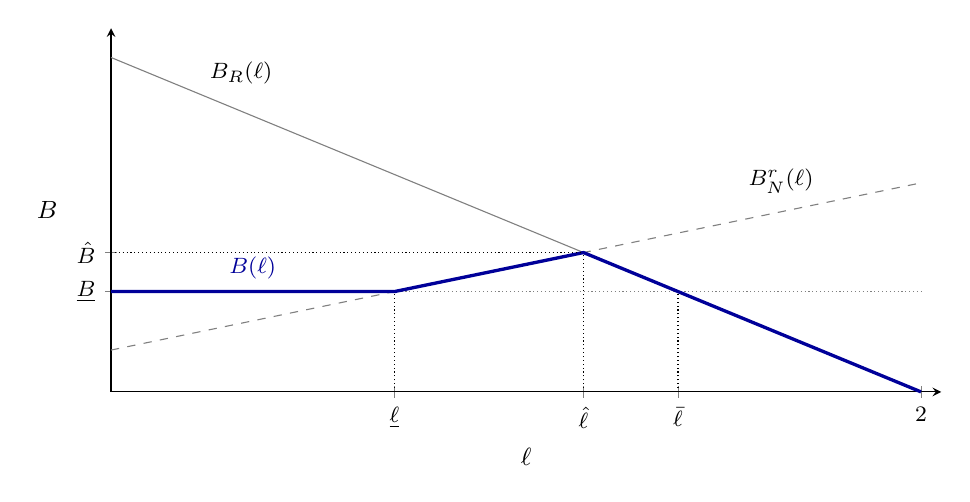
\begin{tikzpicture}
\begin{axis}[
  width=\linewidth, height=6.2cm,
  axis lines=left, xmin=0, xmax=2.05, ymin=0, ymax=1.45,
  xlabel={$\ell$}, ylabel={$B$}, ylabel style={rotate=-90},
  xtick={0.7,1.16667,1.4,2}, xticklabels={$\underline\ell$,$\hat\ell$,$\bar\ell$,$2$},
  ytick={0.4,0.55556}, yticklabels={$\underline B$,$\hat B$},
  tick label style={font=\footnotesize}, label style={font=\small},
  clip=false]
\addplot[domain=0:2, samples=2, dashed, gray] {1/6 + x/3};
\addplot[domain=0:2, samples=2, gray] {4/3 - 2*x/3};
\addplot[domain=0:2, samples=2, densely dotted, gray] {0.4};
\addplot[very thick, blue!60!black] coordinates {(0,0.4) (0.7,0.4) (1.16667,0.55556) (2,0)};
\draw[densely dotted] (axis cs:0.7,0) -- (axis cs:0.7,0.4);
\draw[densely dotted] (axis cs:1.16667,0) -- (axis cs:1.16667,0.55556);
\draw[densely dotted] (axis cs:1.4,0) -- (axis cs:1.4,0.4);
\draw[densely dotted] (axis cs:0,0.55556) -- (axis cs:1.16667,0.55556);
\node[font=\footnotesize, anchor=west] at (axis cs:1.55,0.84) {$B_N^r(\ell)$};
\node[font=\footnotesize, anchor=west] at (axis cs:0.22,1.27) {$B_R(\ell)$};
\node[font=\footnotesize, blue!60!black, anchor=south] at (axis cs:0.35,0.41) {$B(\ell)$};
\end{axis}
\end{tikzpicture}
\caption{The optimal amnesty rate}\label{fig:12-leniency-a}
\end{subfigure}\hfill
\begin{subfigure}[t]{0.49\textwidth}
\centering
\begin{tikzpicture}
\begin{axis}[
  width=\linewidth, height=6.2cm,
  axis lines=left, xmin=0, xmax=2.05, ymin=0, ymax=1.45,
  xlabel={$\ell$}, ylabel={$B$}, ylabel style={rotate=-90},
  xtick={1,1.16667}, xticklabels={$\hat\ell'$,$\hat\ell$},
  ytick={0.55556,0.66667}, yticklabels={$\hat B$,$\hat B'$},
  tick label style={font=\footnotesize}, label style={font=\small},
  clip=false]
\addplot[domain=0:2, samples=2, dashed, gray] {1/6 + x/3};
\addplot[domain=0:2, samples=2, thick, dashed, red!70!black] {1/3 + x/3};
\addplot[domain=0:2, samples=2, gray] {4/3 - 2*x/3};
\draw[densely dotted] (axis cs:1,0) -- (axis cs:1,0.66667) -- (axis cs:0,0.66667);
\draw[densely dotted] (axis cs:1.16667,0) -- (axis cs:1.16667,0.55556) -- (axis cs:0,0.55556);
\draw[-{Stealth[length=2mm]}] (axis cs:1.62,0.72) -- (axis cs:1.47,0.86);
\node[font=\footnotesize, anchor=west] at (axis cs:1.62,0.68) {$B_N^r(\ell;\varrho)$};
\node[font=\footnotesize, red!70!black, anchor=east] at (axis cs:1.45,0.92) {$B_N^r(\ell;\varrho')$};
\node[font=\footnotesize, anchor=west] at (axis cs:0.22,1.27) {$B_R(\ell)$};
\end{axis}
\end{tikzpicture}
\caption{A higher detection probability}\label{fig:12-leniency-b}
\end{subfigure}
\caption{Optimal leniency in the model of \citet{ChenRey2013}, drawn for $\delta = 0.8$ and $F = 1$. Panel (a): with
$\varrho = 0.3$, normal collusion survives above $\max\{\underline B, B_N^r(\ell)\}$ and collude and report survives
above $B_R(\ell)$. The deterrence threshold $B(\ell)$ (thick line) is the lower envelope. It equals
$\underline B = 0.4$ up to $\underline\ell = 0.7$ and peaks at $\hat\ell = \frac{7}{6}$, where
$\hat B = \frac{5}{9}$. Excessive leniency starts at $\bar\ell = 1.4$. Panel (b): raising $\varrho$ from 0.3 to
$\varrho' = 0.4$ shifts $B_N^r$ up and leaves $B_R$ unchanged, so the optimal rate falls to $\hat\ell' = 1$ and the
threshold rises to $\hat B' = \frac{2}{3}$. Redrawn with computed values from \citet{ChenRey2013}, Figures 1 and 2.}
\label{fig:12-leniency}
\end{figure}

\casehead{Interpretation}
\Cref{fig:12-leniency} shows the trade-off. Rates below $\underline\ell$ do nothing, because a deviator would not
report. Rates between $\underline\ell$ and $\hat\ell$ deter normal collusion in more industries, because they make
``cheat and report'' attractive. Rates above $\hat\ell$ hand the cartel a cheaper way to collude, by reporting itself
every period. At $\hat\ell$ the \emph{marginal industry}, with $B = \hat B$, is on the edge of both forms of
collusion. A lower rate would let it collude normally without fear of a reporting deviator. A higher rate would let it
collude and report without fear of a product-market deviator. Chen and Rey describe the instruments as a stick, the
probability $\varrho$ of random detection, and a carrot, the amnesty rate $\ell$. The weaker the stick, the larger
the optimal carrot. With no stick at all ($\varrho = 0$), $\underline\ell = 1$, so a pure fine reduction ($\ell \le 1$)
is useless and only rewards can work \citep[footnote~13]{ChenRey2013}.

Part~(d) of \cref{prop:12-chen-rey} explains why ``collude and report'' is rarely observed even though it is the
constraint that pins down the optimal rate. At the optimal rate, every industry that can collude prefers normal
collusion. The threat of self-reporting cartels shapes the policy without appearing in the data.

\begin{example}[Leniency with numbers]\label{ex:12-leniency-numbers}
Let $\delta = 0.8$, $\varrho = 0.3$ and $F = 1$, as in \cref{fig:12-leniency-a}. Without leniency,
$\underline B = \frac{0.8 \times 0.3}{0.6} = 0.4$. Deviators report once $\ell > 0.7$, and leniency becomes excessive
at $\bar\ell = 1.4$. The optimal rate is $\hat\ell = \frac{0.7}{0.6} = \frac{7}{6}$. The first informant thus pays no
fine and receives a reward of $\frac{1}{6}$ of the fine. The deterrence threshold rises to
$\hat B = \frac{0.8 \times 0.5}{0.6 \times 1.2} = \frac{5}{9} \approx 0.556$. Leniency extends deterrence from
industries with stakes below $0.4F$ to industries with stakes below $0.556F$, a rise of about 39 percent. In
industries that still collude, normal collusion beats collude and report by $\frac{0.7}{1.2}F \approx 0.583F$ per
firm. These values are computed in \texttt{figures/ch12/src/chenrey\_check.py}.
\end{example}

\casehead{Laboratory evidence}
\citet{HinloopenSoetevent2008}, as described by \citet[p.~13]{ChenRey2013}, ran laboratory experiments with
$\varrho = 0.4$ and $\delta = 0.8$. The model then prescribes full amnesty, since $\hat\ell = \frac{1 - 0.4}{1 - 0.4} = 1$.
One treatment set the rate at this level. The other granted full amnesty to a sole reporter and a 90 percent
reduction to each firm when both reported \citep[footnote~14]{ChenRey2013}. Under collude and report each firm then
pays $0.1F = (1 - \frac{\ell}{2})F$, which corresponds to $\ell = 1.8$. Subjects never colluded and reported in the
first treatment. More than 70 percent of subjects did so in every period of the second treatment, as the model
predicts. Our own computation shows how generous the second treatment is. With $\varrho = 0.4$, excessive leniency
starts at $\bar\ell = 1.2$. At $\ell = 1.8$, $B_R = \frac{0.8 \times 0.1}{0.6}F \approx 0.133F$, far below
$\underline B = \frac{0.8 \times 0.4}{0.6}F \approx 0.533F$. The program would make collusion sustainable in industries
that enforcement without leniency deters.

\citet{Spagnolo2004} proposes to reward the first informant with the fines paid by the other cartel members, which
corresponds to $\ell = 2$ in this model. \citet[p.~13]{ChenRey2013} counsel caution, because $\hat\ell < \bar\ell < 2$.
Actual programs grant reductions of up to 100 percent and rarely pay rewards. By \cref{prop:12-chen-rey}, such rates
may lie below the optimum when random detection is weak ($\varrho < \frac{\delta}{2}$).

\begin{remark}[The first-informant rule]\label{rem:12-first-informant}
Suppose both informants receive the reduced fine. Normal collusion is unaffected, because a deviator reports alone.
Under collude and report, however, each firm now pays $(1-\ell)F$ for sure. Repeating the derivation of
\eqref{eq:12-cr-BR} with $(1-\ell)$ in place of $(1 - \frac{\ell}{2})$ gives
\begin{equation}\label{eq:12-cr-BRprime}
B_R'(\ell) = \frac{\delta(1-\ell)}{2\delta - 1}\,F < B_R(\ell).
\end{equation}
At $\ell = \underline\ell = 1 - \varrho$, $B_R'(\underline\ell) = \frac{\delta\varrho F}{2\delta-1} = \underline B$.
For $\ell > \underline\ell$, $B_R'(\ell) < \underline B \le B_N(\ell)$, so the threshold falls below $\underline B$.
For $\ell \le \underline\ell$, the threshold equals $\underline B$. Without the first-informant rule, leniency cannot
raise deterrence at all \citep[pp.~13--14]{ChenRey2013}. The authors suggest that this may explain why the U.S. program
achieved little before its 1993 revision. The point agrees with \citet{Spagnolo2004} and \citet{Harrington2008}.
\end{remark}

\casehead{Repeat offenders}
Some jurisdictions deny leniency to repeat offenders, which seems to block cartels that report every period. Chen and
Rey argue that the restriction backfires. Their argument omits a participation condition. With it the conclusion is
established only when random detection is strong enough.

\begin{proposition}[Once-only leniency, after \citealp{ChenRey2013}, Proposition~2]\label{prop:12-repeat-offenders}
Suppose each industry can obtain leniency only once, and let $\ell \ge 0$. The strategy ``report once and never
again'' is sustainable if and only if $B \ge \underline B$ and
\begin{equation}\label{eq:12-cr-BO}
B \ge B_O(\ell) \equiv \left[(1-\delta)\left(1 - \frac{\ell}{2}\right) + \delta\varrho\right]F .
\end{equation}
The second condition holds at every $B \ge \underline B$ if and only if
$\ell \ge \ell_O \equiv 2\left(1 - \frac{2\delta\varrho}{2\delta - 1}\right)$. If
$\varrho \ge \frac{2\delta - 1}{2\delta + 1}$, then $\ell_O \le \underline\ell$. At every amnesty rate, normal
collusion or report once is then sustainable whenever $B \ge \underline B$. In that case once-only leniency cannot
deter collusion in any industry that enforcement without leniency fails to deter.
\end{proposition}

\begin{proof}
Under ``report once,'' the firms collude in every period, both report in the first period, and nobody reports
afterwards. Each firm's value is
\begin{equation*}
V_O = B - \left(1 - \frac{\ell}{2}\right)F + \delta V_N
= B - \left(1 - \frac{\ell}{2}\right)F + \delta\,\frac{B - \varrho F}{1-\delta}.
\end{equation*}
After the first report, leniency is no longer available. Reporting then only exposes the reporter, so play continues
as normal collusion without leniency. By \cref{prop:12-fines}, it is sustainable if and only if $B \ge \underline B$.
In the first period, reporting is self-enforcing, as under collude and report. A product-market deviator still
reports and pays $(1 - \frac{\ell}{2})F$ in expectation. It earns $2B$ and nothing afterwards. The first-period
constraint is
\begin{align*}
B - \left(1 - \frac{\ell}{2}\right)F + \delta V_N &\ge 2B - \left(1 - \frac{\ell}{2}\right)F\\
\delta\,\frac{B - \varrho F}{1-\delta} &\ge B\\
(2\delta - 1)B &\ge \delta\varrho F,
\end{align*}
which is again $B \ge \underline B$. A firm can also refuse at stage~0 of the first period. No evidence then arises,
the firms compete, and the refusing firm earns zero from then on. Refusal is unprofitable if and only if $V_O \ge 0$.
Multiplying $V_O \ge 0$ by $1 - \delta$ gives $B \ge (1-\delta)(1 - \frac{\ell}{2})F + \delta\varrho F$, which is
\eqref{eq:12-cr-BO}.

For the second claim, \eqref{eq:12-cr-BO} holds at $B = \underline B$ if and only if
\begin{equation*}
(1-\delta)\left(1 - \frac{\ell}{2}\right) \le \frac{\delta\varrho}{2\delta - 1} - \delta\varrho
= \frac{2(1-\delta)\delta\varrho}{2\delta - 1},
\end{equation*}
that is $1 - \frac{\ell}{2} \le \frac{2\delta\varrho}{2\delta - 1}$, or $\ell \ge \ell_O$. Since $B_O$ does not
depend on $B$, the condition then holds at every $B \ge \underline B$. Next, $\ell_O \le \underline\ell = 1 - \varrho$
if and only if $1 + \varrho \le \frac{4\delta\varrho}{2\delta - 1}$, that is $2\delta - 1 \le (2\delta + 1)\varrho$.
Normal collusion is unaffected by the restriction, since it never uses leniency on the path. By
\eqref{eq:12-cr-BN} it is sustainable at every $B \ge \underline B$ when $\ell \le \underline\ell$. Report once covers
every $\ell \ge \ell_O$, and $\ell_O \le \underline\ell$ leaves no gap.
\end{proof}

Chen and Rey check only the product-market constraints of report once, and their Proposition~2 states that the
restriction makes leniency ineffective without qualification \citep[pp.~14--15]{ChenRey2013}. The stage-0 refusal
matters. With $\delta = 0.8$, $\varrho = 0.3$, $F = 1$, $\ell = 0.2$ and $B = \underline B = 0.4$, we get
$V_N = 0.5$ and $V_O = 0.4 - 0.9 + 0.4 = -0.1 < 0$, so report once fails. Normal collusion survives there, because
$\ell = 0.2$ lies below $\underline\ell = 0.7$. In this example $\ell_O = 0.4 < \underline\ell$, and the
conclusion of Chen and Rey holds. When random detection is weak, both strategies can fail at a stake above
$\underline B$. With $\delta = 0.9$ and
$\varrho = 0.1$, $\underline\ell = 0.9$ and $\ell_O = 1.55$. At $\ell = 1.2$ and $B = 0.12F$, above
$\underline B = 0.1125F$, normal collusion needs $B \ge B_N^r(1.2) = 0.15F$ and report once needs
$B \ge B_O(1.2) = 0.13F$. Both fail. These values are our own computations in
\texttt{figures/ch12/src/chenrey\_check.py}. We have not shown that every other collusive strategy fails there too.

The logic of the proposition is that one report uses up the industry's access to leniency. Afterwards no member can
gain from reporting, which removes the threat that made normal collusion fragile. The first report is costly,
however, and a cartel accepts that cost only if the whole path is worth at least the zero it earns by not forming.
Chen and Rey quote \citet{Wils2008} on the same
paradox, that excluding recidivists from leniency may encourage recidivism. When exposed cartels face closer scrutiny
afterwards, excluding repeat offenders still weakens the program but no longer makes it useless
\citep[p.~17]{ChenRey2013}.

\casehead{Closer scrutiny after exposure}
So far an exposed cartel could collude again in the next period. Suppose instead that an exposed industry is kept
under tight supervision for $T$ periods, during which it cannot collude. Define
\begin{equation}\label{eq:12-cr-beta-gamma}
\beta_T \equiv \delta^{T+1}, \qquad \gamma_T \equiv (1-\varrho)\delta + \varrho\beta_T,
\end{equation}
so that $\beta_T < \gamma_T < \delta$ for $T \ge 1$. (Chen and Rey write $\beta(T)$ and $\gamma(T)$.) A cartel that
reports every period is exposed every period, so its future is discounted at $\beta_T$:
\begin{equation*}
V_R(\ell;T) = B - \left(1 - \frac{\ell}{2}\right)F + \beta_T V_R(\ell;T)
\quad\Longrightarrow\quad
V_R(\ell;T) = \frac{B - \left(1 - \frac{\ell}{2}\right)F}{1 - \beta_T}.
\end{equation*}
A normal cartel is exposed only with probability $\varrho$:
\begin{equation*}
V_N(T) = B - \varrho F + (1-\varrho)\delta V_N(T) + \varrho\beta_T V_N(T)
\quad\Longrightarrow\quad
V_N(T) = \frac{B - \varrho F}{1 - \gamma_T}.
\end{equation*}
Repeating the derivations of \eqref{eq:12-fines-threshold}, \eqref{eq:12-cr-BNr} and \eqref{eq:12-cr-BR} with these
values gives
\begin{equation}\label{eq:12-cr-scrutiny}
\underline B(T) = \frac{\gamma_T\varrho F}{2\gamma_T - 1},\qquad
B_N^r(\ell;T) = \frac{\varrho - (1-\gamma_T)(1-\ell)}{2\gamma_T - 1}\,F,\qquad
B_R(\ell;T) = \frac{\beta_T\left(1 - \frac{\ell}{2}\right)}{2\beta_T - 1}\,F.
\end{equation}
The last expression requires $\beta_T > \frac{1}{2}$.\footnote{Footnote~20 of the working paper (p.~16) prints this
assumption as $\beta(T) < \frac{1}{2}$. That inequality contradicts the paper's own formula for $B_R(q;T)$, whose
denominator $2\beta(T) - 1$ must be positive. It also contradicts the footnote's own parenthetical remark, which
treats $\gamma(T) > \frac{1}{2} > \beta(T)$ as the case in which collude and report cannot be sustained. We state the
condition that the formula needs.} If $\beta_T \le \frac{1}{2}$ and $\ell < 2$, collude and report
cannot be sustained at any stake. The authority can then raise the amnesty rate up to that bound without inviting
self-reporting cartels.
Equating $B_N^r(\ell;T)$ and $B_R(\ell;T)$ gives the optimal rate
\begin{equation}\label{eq:12-cr-qhatT}
\hat\ell(T) = \frac{2(1-\varrho)(\beta_T + \delta - 1)}{(2\beta_T - 1) + (2\gamma_T - 1)(1 - \beta_T)},
\end{equation}
which reduces to \eqref{eq:12-cr-qhat} at $T = 0$, where $\beta_0 = \gamma_0 = \delta$.

\begin{proposition}[Scrutiny, \citealp{ChenRey2013}, Proposition~3]\label{prop:12-scrutiny}
Assume $\beta_T > \frac{1}{2}$. A longer period $T$ of close scrutiny for exposed cartels raises the maximal
deterrence threshold $\hat B(T)$ and also raises the optimal amnesty rate $\hat\ell(T)$.
\end{proposition}

Scrutiny lowers the value of both forms of collusion, but it hurts collude and report more, because that cartel is
exposed in every period. The authority can then offer more amnesty without inviting self-reporting cartels. With
$\delta = 0.9$ and $\varrho = 0.2$, for instance, our computations give $\hat\ell = 1.455$ and $\hat B = 0.307F$ at
$T = 0$, $\hat\ell = 1.534$ and $\hat B = 0.371F$ at $T = 2$, and $\hat\ell = 1.873$ and $\hat B = 0.539F$ at
$T = 5$. At $T = 6$, $\beta_T = 0.9^7 < \frac{1}{2}$, and collude and report is no longer sustainable.

\begin{remark}[More than two firms]\label{rem:12-cr-nfirms}
The model extends directly to $N$ firms, an extension we derive here. A deviator earns $NB$, and under collude and
report each firm is the first informant with probability $\frac{1}{N}$, so its expected fine is
$(1 - \frac{\ell}{N})F$. The derivations above give
\begin{equation*}
B_N^r(\ell) = \frac{\varrho - (1-\delta)(1-\ell)}{N\delta - (N-1)}\,F,\qquad
B_R(\ell) = \frac{\delta\left(1 - \frac{\ell}{N}\right)}{N\delta - (N-1)}\,F,
\end{equation*}
and the optimal rate solves $\varrho - (1-\delta) + (1-\delta)\ell = \delta - \frac{\delta\ell}{N}$, so
\begin{equation*}
\hat\ell_N = \frac{1 - \varrho}{1 - \frac{N-1}{N}\delta},\qquad
\hat B_N = \frac{\delta[(N-1)(1-\delta) + \varrho]}{[N\delta - (N-1)][N(1-\delta) + \delta]}\,F.
\end{equation*}
Excessive leniency starts at $\bar\ell_N = N(1-\varrho)$. Both $\hat\ell_N$ and $\bar\ell_N$ rise with $N$. A reporting
cartel with many members spreads the amnesty thinly, so the authority can afford a larger reward. With $\delta = 0.9$
and $\varrho = 0.3$, $\hat\ell_N$ equals 1.27, 1.75 and 2.15 for $N = 2$, 3 and 4. This extension keeps the restriction
to the two strategies N and R.
\end{remark}

\casehead{Leniency before and after an investigation}
The final part of \citet[Section~4]{ChenRey2013} separates the launch of an investigation from its outcome. Absent any
report, the authority opens an investigation with probability $\iota \in (0,1)$. An open investigation uncovers the
cartel, absent any report, with probability $\varsigma \in (0,1)$. (Chen and Rey write $\alpha$ and $p$.) Both
probabilities are likely to be small in practice. If investigations are secret, firms face the overall detection
probability $\varrho = \iota\varsigma$, and \cref{prop:12-chen-rey} applies with this $\varrho$. If the rates before
and after an investigation differ, the relevant secret rate is the expected one, $\iota\ell_a + (1-\iota)\ell_b$
\citep[footnote~22]{ChenRey2013}.

If investigations are public, the authority can set two rates. A first informant pays $(1-\ell_b)F$ if it reports
before an investigation and $(1-\ell_a)F$ if it reports after one has opened. Stages~0 to~2 are as before. At
stage~3, if nobody has reported, the authority opens an investigation with probability $\iota$. At stage~4 the firms
may report again, and an unreported cartel under investigation is uncovered with probability $\varsigma$. Public investigations create a third collusive strategy, \emph{collude and report if
investigated} (I).

The authority can always do as well with public investigations as with secret ones, by setting $\ell_a = 0$. A report
after an investigation then raises the probability of conviction from $\varsigma$ to 1 without reducing the fine, so
nobody reports at stage~4. The choice between N and R is then the same as with secret investigations. The question is
whether $\ell_a > 0$ can do strictly better.

Each strategy faces several deviations, and we derive each threshold from a comparison of values. Normal collusion now
has value $V_N = \frac{B - \iota\varsigma F}{1-\delta}$. It must deter four deviations. Deviating without reporting
gives $\underline B = \frac{\delta\iota\varsigma F}{2\delta - 1}$. Deviating and reporting at stage~2 gives
$B_N^r(\ell_b) = \frac{\iota\varsigma - (1-\delta)(1-\ell_b)}{2\delta - 1}F$. Deviating and reporting only if
investigated yields $2B - \iota(1-\ell_a)F$, and $V_N \ge 2B - \iota(1-\ell_a)F$ gives
\begin{equation*}
B \ge B_N^i(\ell_a) \equiv \frac{\iota\varsigma - \iota(1-\delta)(1-\ell_a)}{2\delta - 1}\,F.
\end{equation*}
Colluding but reporting once an investigation opens compares $-\varsigma F + \delta V_N$ (stay silent and keep the
cartel) with $-(1-\ell_a)F$ (report and lose it). Staying silent is better if and only if
\begin{equation*}
B \ge B_N^c(\ell_a) \equiv \frac{\varsigma(1 - \delta + \iota\delta) - (1-\delta)(1-\ell_a)}{\delta}\,F.
\end{equation*}
Normal collusion is therefore sustainable if and only if
\begin{equation}\label{eq:12-cr-open-N}
B \ge B_N(\ell_b, \ell_a) \equiv \max\{B_N^i(\ell_a),\, B_N^r(\ell_b),\, B_N^c(\ell_a),\, \underline B\},
\end{equation}
equation~(6) of \citet{ChenRey2013}. Collude and report is sustainable if and only if
$B \ge B_R(\ell_b) = \frac{\delta(1 - \frac{\ell_b}{2})F}{2\delta-1}$, as before. Under collude and report if
investigated, each firm pays $(1 - \frac{\ell_a}{2})F$ when an investigation opens, so
$V_I = \frac{B - \iota(1 - \frac{\ell_a}{2})F}{1-\delta}$. Reporting when investigated is self-enforcing, since it cuts
the expected fine from $F$ to $(1 - \frac{\ell_a}{2})F$ when the rival reports. Strategy I must deter a deviation with
a report at stage~2, which yields $2B - (1-\ell_b)F$, and a deviation with a report only if investigated, which yields
$2B - \iota(1 - \frac{\ell_a}{2})F$. These give
\begin{equation}\label{eq:12-cr-open-I}
B \ge B_I(\ell_b, \ell_a) \equiv \max\left\{
\frac{\delta\iota\left(1 - \frac{\ell_a}{2}\right)}{2\delta - 1}\,F,\;
\frac{\iota\left(1 - \frac{\ell_a}{2}\right) - (1-\delta)(1-\ell_b)}{2\delta - 1}\,F\right\},
\end{equation}
where the two terms are $B_I^i(\ell_a)$ and $B_I^r(\ell_b, \ell_a)$, equation~(7) of \citet{ChenRey2013}. The
authority maximizes $\min\{B_N(\ell_b,\ell_a),\, B_I(\ell_b,\ell_a),\, B_R(\ell_b)\}$. Without post-investigation
leniency, the optimum is $\ell_b = \hat\ell(\iota\varsigma)$ with threshold $\hat B(\iota\varsigma)$, from
\eqref{eq:12-cr-qhat} and \eqref{eq:12-cr-Bhat}.

Post-investigation leniency can destabilize normal collusion in two ways. The first route makes ``deviate and report
if investigated'' the binding deviation. This requires $B_N^i(\ell_a) > B_N^r(\hat\ell_b)$, that is,
$\iota(1-\ell_a) < 1 - \hat\ell(\iota\varsigma)$. It must not make strategy I more robust, which requires
$B_I^r(\hat\ell_b, \ell_a) > B_N^r(\hat\ell_b)$, that is, $\varsigma < 1 - \frac{\ell_a}{2}$. Both conditions hold for
some $\ell_a$ if and only if
\begin{equation}\label{eq:12-cr-p1}
\varsigma < \tilde\varsigma_1(\iota) \equiv \frac{\iota(2-\delta) - \delta}{2\iota(1-\delta)},
\end{equation}
equation~(9) of \citet{ChenRey2013}. To verify it, substitute $1 - \hat\ell(\iota\varsigma) =
\frac{2\iota\varsigma - \delta}{2-\delta}$ into the first condition and combine it with $\ell_a < 2(1-\varsigma)$.
Then reduce $\ell_b$ slightly below $\hat\ell$ to raise $B_R$ as well. The best policy of this kind equalizes the three
binding thresholds, $B_N^i(\tilde\ell_a^1) = B_I^r(\tilde\ell_b^1, \tilde\ell_a^1) = B_R(\tilde\ell_b^1)$, which gives
\begin{equation}\label{eq:12-cr-policy1}
\tilde\ell_b^1 = \frac{2[(1-\iota)(2-\delta) + \iota(1-\varsigma)]}{2(1-\delta)^2 + 2 - \delta},\qquad
\tilde\ell_a^1 = \frac{2}{\iota}\cdot\frac{\delta(1-\delta)(1-\iota) + \iota(1-\varsigma)(2-\delta)}{2(1-\delta)^2 + 2 - \delta},
\end{equation}
and the deterrence threshold
\begin{equation}\label{eq:12-cr-B1}
\tilde B_1 = \frac{2(1-\delta)^2 + \iota(1 - \delta + \varsigma)}{2(1-\delta)^2 + 2 - \delta}\cdot\frac{\delta F}{2\delta - 1},
\end{equation}
equations~(10) and~(11) of \citet{ChenRey2013}. It exceeds $\hat B(\iota\varsigma)$ if and only if
$\varsigma \le \tilde\varsigma_1(\iota)$. The second route makes ``collude but report if investigated'' the binding
deviation. It is available if and only if
\begin{equation}\label{eq:12-cr-p2}
\varsigma \le \tilde\varsigma_2(\iota) \equiv \frac{(1-\delta)(3\delta - 2)}{(2\delta - 1)(2-\delta) + 2\iota\delta(1-\delta)},
\end{equation}
which is positive only when $\delta > \frac{2}{3}$. Its best version $(\tilde\ell_b^2, \tilde\ell_a^2)$ equalizes
$B_N^c$, $B_I^r$ and $B_R$, with threshold
\begin{equation}\label{eq:12-cr-B2}
\tilde B_2 = \frac{2(1-\delta)^2 + \iota(1-\delta) + (1 - \delta + \iota\delta)\iota\varsigma}
{2(2\delta - 1)(1-\delta)(2-\delta) + \iota\delta^2}\,\delta F,
\end{equation}
equations~(12) to~(14) of \citet{ChenRey2013}. The first route beats the second if and only if
$\varsigma \ge \tilde\varsigma(\iota)$, where
\begin{equation}\label{eq:12-cr-ptilde}
\tilde\varsigma(\iota) \equiv \frac{2(1-\delta)(2\delta - 1) + \iota(2\delta^2 - 1) - \iota^2\delta}
{\iota(2\delta - 1)(3 - 2\delta) + 4\iota^2(1-\delta)^2},
\end{equation}
which is nonpositive for $\iota \ge \iota_1 \equiv \frac{2\delta - 1}{\delta}$. We checked every formula in this
paragraph symbolically in \texttt{chenrey\_check.py}.

\begin{proposition}[Pre- and post-investigation leniency, \citealp{ChenRey2013}, Proposition~4]\label{prop:12-cr-open}
It is always optimal to offer leniency before an investigation.
\begin{enumerate}[label=(\alph*)]
\item If firms are patient ($\delta > \frac{2}{3}$), it is optimal to keep offering some leniency once an investigation
is under way if and only if $\varsigma \le \max\{\tilde\varsigma_1(\iota), \tilde\varsigma_2(\iota)\}$. The optimal
policy is then $(\tilde\ell_b^1, \tilde\ell_a^1)$ if $\varsigma \ge \tilde\varsigma(\iota)$ and
$(\tilde\ell_b^2, \tilde\ell_a^2)$ if $\varsigma \le \tilde\varsigma(\iota)$.
\item If firms are less patient ($\frac{1}{2} < \delta \le \frac{2}{3}$), it is optimal to keep offering some leniency
once an investigation is under way if and only if $\iota \ge \underline\iota \equiv \frac{\delta}{2-\delta}$ and
$\varsigma \le \tilde\varsigma_1(\iota)$. The optimal policy is then $(\tilde\ell_b^1, \tilde\ell_a^1)$.
\end{enumerate}
In all other cases the optimal policy is $(\hat\ell(\iota\varsigma), 0)$.
\end{proposition}

\begin{figure}[htbp]
\centering
\begin{subfigure}[t]{0.49\textwidth}
\centering
\begin{tikzpicture}
\begin{axis}[
  width=\linewidth, height=6cm,
  axis lines=left, xmin=0, xmax=1.03, ymin=0, ymax=1.03,
  xlabel={$\iota$}, ylabel={$\varsigma$}, ylabel style={rotate=-90},
  xtick={0,0.666667,1}, xticklabels={$0$,$\frac{2}{3}$,$1$},
  ytick={0,0.2,1}, yticklabels={$0$,$0.2$,$1$},
  tick label style={font=\footnotesize}, label style={font=\small},
  clip=false]
\addplot[thick, domain=0:0.686141, samples=60] {1/(9+4*x)};
\addplot[thick, domain=0.686141:1, samples=120] {3-2/x};
\addplot[thick, dashed, domain=0.686141:0.75, samples=60] {(6+7*x-20*x^2)/(21*x+4*x^2)};
\draw[densely dotted, gray] (axis cs:0,0.2) -- (axis cs:1,0.2);
\node[font=\small] at (axis cs:0.40,0.55) {A};
\node[font=\small] at (axis cs:0.92,0.30) {B};
\node[font=\footnotesize, anchor=east] at (axis cs:0.86,0.75) {$\tilde\varsigma_1(\iota)$};
\node[font=\footnotesize, anchor=south west] at (axis cs:0.04,0.115) {$\tilde\varsigma_2(\iota)$};
\end{axis}
\end{tikzpicture}
\caption{The unit square}\label{fig:12-leniency-regions-a}
\end{subfigure}\hfill
\begin{subfigure}[t]{0.49\textwidth}
\centering
\begin{tikzpicture}
\begin{axis}[
  width=\linewidth, height=6cm,
  axis lines=left, xmin=0, xmax=1.03, ymin=0, ymax=0.206,
  xlabel={$\iota$}, ylabel={$\varsigma$}, ylabel style={rotate=-90},
  xtick={0,0.666667,0.75,1}, xticklabels={$0$,$\frac{2}{3}$,$\frac{3}{4}$,$1$},
  ytick={0,0.085,0.111111,0.2}, yticklabels={$0$,$\varsigma_0$,$\frac{1}{9}$,$0.2$},
  tick label style={font=\footnotesize}, label style={font=\small},
  clip=false]
\addplot[thick, domain=0:0.686141, samples=60] {1/(9+4*x)};
\addplot[thick, domain=0.686141:0.714286, samples=60] {3-2/x};
\addplot[thick, dashed, domain=0.686141:0.75, samples=60] {(6+7*x-20*x^2)/(21*x+4*x^2)};
\draw[densely dotted] (axis cs:0,0.085) -- (axis cs:0.686,0.085);
\node[font=\small] at (axis cs:0.35,0.165) {A};
\node[font=\small] at (axis cs:0.88,0.10) {B};
\node[font=\small] at (axis cs:0.35,0.045) {C};
\node[font=\footnotesize, anchor=east] at (axis cs:0.69,0.18) {$\tilde\varsigma_1(\iota)$};
\node[font=\footnotesize, anchor=south] at (axis cs:0.30,0.104) {$\tilde\varsigma_2(\iota)$};
\node[font=\footnotesize, anchor=west] at (axis cs:0.76,0.055) {$\tilde\varsigma(\iota)$};
\draw[-{Stealth[length=1.5mm]}] (axis cs:0.765,0.05) -- (axis cs:0.73,0.03);
\end{axis}
\end{tikzpicture}
\caption{Detail for $\varsigma \le 0.2$}\label{fig:12-leniency-regions-b}
\end{subfigure}
\caption{Optimal leniency policies with public investigations for $\delta = 0.8$, computed from
\eqref{eq:12-cr-p1}, \eqref{eq:12-cr-p2} and \eqref{eq:12-cr-ptilde}. The horizontal axis is the probability $\iota$
that an investigation opens, and the vertical axis the probability $\varsigma$ that it succeeds without a report.
Here $\tilde\varsigma_1(\iota) = 3 - \frac{2}{\iota}$ and $\tilde\varsigma_2(\iota) = \frac{1}{9 + 4\iota}$, and the
three curves meet at $\iota_0 \approx 0.686$, $\varsigma_0 \approx 0.085$. In region A no leniency is offered after an
investigation opens. In region B the optimal policy is $(\tilde\ell_b^1, \tilde\ell_a^1)$, and in region C it is
$(\tilde\ell_b^2, \tilde\ell_a^2)$. Panel (b) enlarges the strip $\varsigma \le 0.2$ of panel (a). Redrawn with
computed boundaries from \citet{ChenRey2013}, Figure~4.}
\label{fig:12-leniency-regions}
\end{figure}

\Cref{fig:12-leniency-regions} draws the regions for $\delta = 0.8$. Post-investigation leniency pays when an
investigation, once opened, is unlikely to succeed without a report. It also needs investigations to be frequent
enough for the threat of one to matter at the margin. If deviations in the product market are detected quickly, a
deviator cannot wait for an investigation before reporting. Then only the second route remains, and
post-investigation leniency is optimal if and only if $\varsigma \le \tilde\varsigma_2(\iota)$
\citep[footnote~26]{ChenRey2013}.

\begin{proposition}[Comparative statics, \citealp{ChenRey2013}, Propositions~5 and~6]\label{prop:12-cr-statics}
\leavevmode
\begin{enumerate}[label=(\alph*)]
\item A higher $\varsigma$ or a higher $\iota$ makes the leniency program more effective.
\item A higher $\varsigma$ calls for less leniency both before and after an investigation.
\item A higher $\iota$ calls for less leniency before an investigation. The post-investigation rate $\tilde\ell_a^1$
falls with $\iota$, while $\tilde\ell_a^2$ rises with $\iota$.
\item Offering post-investigation leniency lowers the pre-investigation rate: $\tilde\ell_b^1 < \hat\ell$ and
$\tilde\ell_b^2 < \hat\ell$.
\item More leniency is offered after than before an investigation when investigations are unlikely to succeed:
$\tilde\ell_b^1 < \tilde\ell_a^1$ if and only if $\varsigma < \hat\varsigma_1(\iota)$, and $\tilde\ell_b^2 <
\tilde\ell_a^2$ if and only if $\varsigma < \hat\varsigma_2(\iota)$, where
\begin{equation*}
\hat\varsigma_1(\iota) = (1-\delta)\,\frac{\iota^2 + \delta(1-\iota)}{\iota(2 - \delta - \iota)},\qquad
\hat\varsigma_2(\iota) = \frac{1-\delta}{2\delta - 1}\cdot\frac{\delta(1-\delta) + \iota(2\delta - 1)}{(1 - \delta + \iota\delta)(2 - \delta - \iota)}.
\end{equation*}
\end{enumerate}
\end{proposition}

Part~(d) has a simple logic. Without post-investigation leniency, the marginal industry is on the edge of both normal
collusion and collude and report. Post-investigation leniency destabilizes normal collusion further, and the
pre-investigation rate must then fall to keep collude and report in check. Part~(e) speaks to actual programs. The U.S.
program offers complete amnesty to the first qualifying informant whether or not an investigation is under way, with
further conditions once one has begun. The EU's 1996 notice granted 75 to 100 percent before an investigation and only
50 to 75 percent after. Neither offered more leniency after an investigation opened. \citet[p.~29]{ChenRey2013} conclude that such policies may not be optimal when investigations
rarely succeed without a report.

\casehead{Interpretation}
The model gives sharp answers to the policy questions of \cref{sec:12-legal}. Some leniency always helps, and the
optimal amount falls as random detection improves. Leniency should go to the first informant only. Excluding repeat
offenders can disable the program, at least when random detection is not too weak. Leniency after an investigation opens is valuable when investigations alone rarely
uncover cartels, which is the realistic case. In repeated-game terms, leniency adds the deviation ``cheat and
report'' to the incentive constraint, and its generosity is limited by a second constraint for cartels that report
themselves.

\casehead{Critiques and limitations}
The model is deliberately stark, and several of its simplifications matter.
\begin{enumerate}[label=(\arabic*)]
\item Conduct is binary. With a continuum of collusive prices, leniency would also change the price that a cartel
sets, as \citet[footnote~7]{ChenRey2013} acknowledge.
\item Evidence lasts one period, so a cartel cannot be prosecuted for past conduct. Real fines grow with the duration
of the infringement, and past evidence accumulates. Detection risk then changes over time, which creates a ``race to
the courthouse'' when an investigation looms. \citet{Harrington2008} models this race. With a detection probability
that changes stochastically over time, leniency has two opposing effects \citep[p.~209]{AskerNocke2021}. The
\emph{deviator amnesty effect} lets a member that has just undercut its rivals also report the cartel and escape the
fine, which tightens the no-cheating constraint. The \emph{cartel amnesty effect} lowers the expected fines that
members pay, which raises the value of colluding. A more lenient program can also trigger a switch from no firm
applying to all firms racing to apply, which raises expected fines.
\item The probabilities $\varrho$, $\iota$ and $\varsigma$ are exogenous. Reports free investigative resources, and
\citet{MottaPolo2003} study how an authority allocates a budget between investigation and prosecution. Detection may
also depend on conduct, since price wars and abrupt price rises draw attention.
\item Firms are symmetric. A member that plans to exit, or one with little to lose, has a stronger motive to report.
Asker's weak ring members (\cref{sec:13-asker}) illustrate how asymmetries shape the threat of reporting.
\item Only firms are sanctioned and rewarded. \citet{AubertReyKovacic2006} argue that rewards to individual employees
can deter more effectively. Prison terms for executives make schemes of taking turns at reporting unattractive, as
Wils notes in the passage quoted by \citet[p.~2]{ChenRey2013}.
\item The evidence is mostly experimental. Field evaluation is hard, because the number of detected cartels rises both
when leniency destabilizes cartels and when more cartels form or report themselves. \citet{HarringtonChang2009} build
a model of cartel birth and death to evaluate policy from detected cartels, and \cref{prop:13-selection} shows how
detection shapes the cartels we observe.
\end{enumerate}

\casehead{Contribution}
\citet{ChenRey2013} turn an informal worry into a tractable design problem. The optimal amnesty rate balances two
incentive constraints, one for cartels that fear a reporting deviator and one for cartels that report themselves. The
framework rationalizes the first-informant rule and post-investigation amnesty, the two innovations of the 1993 U.S.
revision. It also warns against generous rewards and against excluding repeat offenders.

\subsection{The agreement requirement: Kaplow (2013)}\label{sec:12-kaplow}

\citet{Kaplow2013} questions the legal foundation on which this enforcement rests. Under Section~1 of the Sherman Act
and Article~101, liability for price fixing requires an agreement among competitors. The conventional view
distinguishes \emph{pure interdependence}, in which firms refrain from price cutting because each expects
retaliation, from classic cartels, whose members meet in hotel rooms to discuss prices. It treats the first as
insufficient for liability and the second as more than sufficient (p.~4). Since the \textit{Theatre Enterprises} decision, courts
have held conscious parallelism by itself to be insufficient. A plaintiff must also show ``plus factors'', such as
actions contrary to the defendants' interests if taken independently and a motive to agree (pp.~109--110). On the
conventional view an agreement turns on the use of certain interfirm communications (p.~21). Kaplow argues that this
focus is misplaced. The harm from coordinated price elevation depends on the extent and duration of supracompetitive
pricing, not on the means used to reach or maintain the understanding (pp.~9--10). That harm is the same whether
firms coordinate in a hotel room or by reading one another's prices.

The repeated-game theory of this chapter supports the premise. In the perfect-monitoring supergames of
\cref{sec:12-perfect}, tacit and explicit collusion are the same equilibrium. The incentive constraint of
\cref{prop:12-bertrand} does not mention communication, and talk is cheap. If communication changes anything, it
selects among the many sustainable prices of \cref{cor:12-bertrand-any-price}.

A test based on communications is hard to state (ch.~3). In its ordinary meaning, communication is any exchange of
information through a common system of symbols, signs or behavior (p.~51). Price moves are behavior conveyed by
signs, so a rule triggered by any communication would cover all interdependent pricing (p.~52). A narrower rule must
count only some communications. It could limit them by mode, counting meetings and emails and excluding hand
signals. It could limit them by content, counting talk about future prices and excluding talk about current ones. Or
it could limit them by setting, counting hotel rooms and excluding public announcements. Modes of communication are close substitutes, however. A fixed list of forbidden modes invites
circumvention, and a rule that includes all functional equivalents covers every successful interdependence
(p.~53). Kaplow draws a striking conclusion. If liability requires certain communications, then ``truly naked price
fixing is per se legal,'' and illegality flows from the communications that clothe it (p.~61).

Noncooperative game theory has no word for agreement, but its central concept is close to the legal one
(pp.~196--199). Courts and dictionaries often define an agreement as a meeting of the minds. An equilibrium of a
repeated game is a mutual understanding about current prices and about the consequences of defection. In any
equilibrium each firm acts in its own interest, given what it expects its rivals to do. A nonbinding agreement that
is not in every member's interest is not honored, so it is not an equilibrium. In Kaplow's words, ``All nonbinding
agreements that work are equilibria, and all equilibria are nonbinding agreements that work'' (p.~197). Not every
equilibrium is objectionable. In repeated static play, no firm refrains from cutting its price because it expects
others to respond, so that equilibrium needs no meeting of the minds (pp.~197--198). Kaplow therefore reads
agreement as successful oligopolistic interdependence, the firms' mutual understanding that sustains
supracompetitive prices (pp.~198--199). On this reading the legal notion maps onto the most collusive equilibria of
\cref{sec:12-folk}.

Communications do not appear in the theory of oligopoly, yet they can matter in two ways (pp.~199--204). The first is
equilibrium selection. Without words, firms may settle on the monopoly price as a focal point, or they may not.
Negotiation helps when the firms disagree about the monopoly price because their costs or their views of demand
differ, and when they sell several products. It can also fail where simple price signaling would quickly converge on
a round number (pp.~200--201). The experimental evidence that Kaplow cites is mixed. In one coordination game,
players reached the good equilibrium 48 percent of the time without communication, 55 percent with two-way
communication and 95 percent with one-way communication (p.~201, note~54). The second role is enforcement when
prices are unobservable. Firms that infer cheating from their own sales risk accidental price wars, and credible
information can avoid them. Cheap talk about compliance is not credible, so verification, such as audits of
invoices, matters more than talk (pp.~202--203). Communication can also hurt a cartel. If firms expect to negotiate
an end to any price war, punishments become brief and cheating more attractive (p.~203). Kaplow concludes that
communications help explain coordinated pricing but do not illuminate the notion of agreement (p.~206). He reaches
the same conclusion about promises and assurances (pp.~206--214).

Kaplow points to what he calls the \emph{paradox of proof} (pp.~6--7 and ch.~6). It arises from two features of the
conventional rule. Agreement requires more than successful interdependence, for example the use of certain
communications. And because firms hide their communications, the factfinder must infer them from circumstantial
evidence, notably from how conducive market conditions are to coordination. Conditions such as few sellers,
homogeneous products and transparent prices make successful price elevation more likely. Beyond some point, they
also make it more likely that firms coordinated without the prohibited means of communication. Evidence of a
greater danger of coordinated pricing can thus reduce the likelihood that an agreement, in the legal sense, exists
(p.~7). A rule that turns on communication tends to exonerate the industries where collusion is most likely.

A stylized calculation of our own, not taken from Kaplow, makes the point concrete. Consider a duopoly with stake
$B \ge \underline B$, so that collusion is sustainable with or without fines. Without communication its firms reach
the collusive equilibrium with probability $\zeta \in [0,1]$ and otherwise compete forever. The parameter $\zeta$
measures how easy tacit coordination is. With communication they always coordinate, but they
face the expected fine $\varrho F$ per period of \cref{sec:12-fines}. Firms communicate if and only if
\begin{equation}\label{eq:12-kaplow}
\frac{B - \varrho F}{1-\delta} > \frac{\zeta B}{1-\delta}
\iff \zeta < 1 - \frac{\varrho F}{B}.
\end{equation}
Industries where tacit coordination is easy collude silently and face no sanction. Industries where it is hard
communicate and are exposed to fines. Tougher enforcement of the agreement requirement lowers the cutoff in
\eqref{eq:12-kaplow}. The industries it moves switch from explicit to tacit collusion. They still collude with
probability $\zeta$, so enforcement deters collusion in them only with probability $1 - \zeta$. The sanction falls
where collusion would otherwise be least likely.

Kaplow proposes a \emph{direct approach}, in which liability turns on evidence that firms engaged in successful
coordinated price elevation, whatever the means (pp.~9--15). Such evidence includes price increases not matched
by changes in cost, price wars, markups estimated from prices and marginal costs or from demand elasticities, and
the conduciveness of market conditions (p.~11). Internal evidence, including interfirm communications, remains
relevant as one source of proof (p.~12). Liability and sanctions should be set by weighing deterrence benefits
against the chilling of desirable behavior and the costs of administration (p.~10). Kaplow argues that, if the
burden of proof under the direct approach is set to find liability in as many cases as the conventional rule, the
direct approach dominates. It targets cases with greater social danger and a lower risk of chilling (p.~14). The
debate is old. \citet{Turner1962} accepted that interdependence could count as agreement as a matter of statutory
language, but rejected it as a basis for liability as a matter of policy. \citet{Posner1969} first argued that this
policy analysis was unsound \citep[p.~447]{Kaplow2013}.

The theory of this chapter gives precise content to Kaplow's second role and so gives reasons to treat
communication as more than a proxy. When information is private, communication changes what can be sustained. In the
model of \citet{HarringtonSkrzypacz2011}
(\cref{thm:12-hs}), sales reports and transfers make collusion possible when unobserved prices would otherwise
undermine it. Without communication, the optimal scheme of \citet{AtheyBagwellSanchirico2004} uses rigid prices and
gives up productive efficiency (\cref{sec:12-private-costs}). With communication about costs, \citet{AtheyBagwell2001}
show that cartels can do better. Explicit agreements may thus raise prices in markets where tacit coordination would
fail. An outcome-based rule faces a measurement problem as well. It must show that prices exceed a noncooperative
benchmark, the identification problem of \cref{ch:conduct}. Conduct that varies with demand, as in the Corts critique
\citep{Corts1999}, makes that benchmark hard to estimate. The detection methods of \cref{ch:collusion-evidence} show
both what such evidence can achieve and how often it is ambiguous.

\section{What Determines Cartel Success?}\label{sec:12-success}

Theory tells us which collusive outcomes can be sustained. It does not tell us how often cartels form, how long they
last, or why they end. \citet{LevensteinSuslow2006} survey the empirical studies of explicit cartels to answer four
questions (p.~43). Can cartels succeed? If so, for how long? What impact do they have? What causes them to break up?
Their survey combines cross-section studies of many cartels with nineteen case studies of individual industries. It is
the main bridge between the theory of this chapter and the evidence of \cref{ch:collusion-evidence}. Page references
are to the journal article.

\subsection{Theory and measurement}\label{sec:12-ls-measure}

\citet[p.~45]{LevensteinSuslow2006} organize the theory around three problems. A cartel must \emph{coordinate} its
members on a collusive outcome and a division of profits, often among multiple equilibria. It must deter
\emph{cheating}. It must prevent \emph{entry} by outsiders attracted by high prices. The theoretical literature
concentrates on cheating, and they summarize it with the $N$-firm Bertrand constraint of \cref{prop:12-bertrand},
whose threshold rises with the number of firms (p.~46). They distinguish two kinds of price war. A punishment war, as
in \citet{GreenPorter1984}, sustains collusion. A breakdown, as in \citet{Stigler1964}, ends it. Following Levenstein's
work on bromine, they add \emph{bargaining price wars}, which erupt when members disagree over the terms of the
agreement after conditions change (p.~56). Entry, finally, is largely ignored by the models even though it is one of
the largest challenges cartels face (p.~49).

The survey covers explicit, ``hard core'' agreements to fix prices or divide markets, both legal and illegal
(p.~49, footnote~18). It excludes state-run cartels such as OPEC and tacit collusion. The cross-section studies fall
into four groups (pp.~49--50): cartels convicted by antitrust authorities, legal international cartels, legal
national cartels, and legal export cartels. The nineteen case studies were chosen for the quality of the analysis,
not at random (footnote~19).

Duration is the most common measure of success because it is the easiest to observe (p.~50). It is a poor measure of
economic impact. Some cartels survive on paper with little effect on prices. Dating is also hard. Suslow, who dates
the end of a cartel by a specific event that ends or restructures it, finds the shortest average duration, 3.7 years.
This suggests that dates of formal dissolution overstate the economic life of cartels (p.~50). Many cartels form,
break down and re-form. Table~3 of \citet{LevensteinSuslow2006} lists such on-and-off episodes for aluminum, coffee,
copper, steel, sugar, sulfur and tin. In copper each episode lasted longer than the one before, a pattern suggestive
of learning (p.~55). The empiricist must decide whether she observes one long cartel or several short ones, and the
answer depends on whether the intervening price wars are punishments or breakdowns. Prosecutions add their own
artifacts. In plea bargains the government announces a continuous cartel period, so the on-and-off pattern disappears
from the record (p.~55, footnote~37).

Every sample is selected. Cross-sections of convicted cartels are, in the authors' words, ``literally selected by
prosecutors'' (p.~44). Legal cartels reflect the legal regime of their time and place. Case studies reflect which
records survived and which histories interested researchers. \Cref{prop:13-selection} shows how detection can bias
the duration of observed cartels in either direction.

\subsection{How long cartels last}\label{sec:12-ls-durations}

\Cref{tab:12-ls-duration} reproduces the cross-section evidence. Average duration ranges from 3.7 to 10 years (p.~50).
The standard deviation within studies ranges from 2.4 to 6.3 years. About half of the cartels lasted less than five
years, but between 12 and 37 percent lasted ten years or more (p.~54). Durations range from less than one year to 29
years. The longest average, 10 years, comes from Japanese export cartels that the state actively supported.

\begin{table}[!tb]
\centering
\caption{Cartel duration in cross-section studies}\label{tab:12-ls-duration}
\footnotesize
\begin{tabular}{@{}l r >{\raggedright\arraybackslash}p{3.8cm} r r r r r@{}}
\toprule
Study & Cartels & Sample & Mean & S.d. & Range & \makecell[r]{Under\\5 yrs (\%)} & \makecell[r]{10 yrs or\\more (\%)}\\
\midrule
Eckbo, sample 1$^{a,c}$ & 23 & International cartels, 1819--1964 & 3.8 & 2.4 & 1--18 & 60 & 12\\
Eckbo, sample 2$^{a,c}$ & 29 & International cartels, 1819--1964 & 4.6 & 4.7 & 0--18$^{d}$ & 57 & 18\\
Griffin, Marquez$^{b}$ & 54 & International cartels, 1888--1984 & 7.3 & 6.3 & 1--29 & 43 & 32\\
Suslow$^{e}$ & 71 & International cartels, 1920--1939 & 3.7 & 3.0 & 1--13 & 40 & 37\\
Posner$^{f}$ & 989 & U.S. Department of Justice cases, 1890--1969 & 7.5 & & & & \\
Dick$^{g}$ & 125 & Webb-Pomerene export associations, 1918--1965 & 5.3 & & & 39 & 24\\
Gallo et al. & 1348 & U.S. Department of Justice cases, 1955--1997 & 5.4 & & & & \\
Jacquemin et al. & 40 & Japanese export cartels, 1967--1972 & 10 & 4.5 & 1--19 & 12.5 & 37.5\\
Levenstein and Suslow & 42 & International cartels, 1990s & 5 & 4.5 & 0--20 & & \\
\bottomrule
\end{tabular}

\smallskip
\begin{minipage}{\textwidth}\footnotesize
Notes: Durations in years. Blank cells are not reported. The table transposes Table~1 of
\citet{LevensteinSuslow2006}, p.~51, where the studies are columns. (a) Excludes an iodine cartel lasting
sixty-one years. (b) Marquez uses Griffin's sample without two episodes (54 versus 52). (c) Eckbo calls a cartel
efficient if it raised price 200 percent above the unit cost of production and distribution. Efficient cartels lasted
5 years on average in sample 1 and 8 years in sample 2, inefficient ones 3.1 and 2.7 years. (d) Episodes shorter than
a year are coded 0. (e) The mean over all 71 episodes is 8.3 years (s.d.\ 6.2). The reported mean is for the 28
episodes not censored by World War II. (f) Posner reports durations only for cases from 1950--1969. (g) Median, from
survival probabilities. Dick reports a median of about 4.5 years for cartels operating common sales agencies and 7.4
years for cartels whose members shipped individually.
Source: \citet{LevensteinSuslow2006}, Table~1.
\end{minipage}
\end{table}

The duration story is similar for contemporary international cartels (p.~52). The authors' own sample covers 42
cartels prosecuted in the 1990s by the United States or the European Commission. In Table~1 it has a mean duration of
5 years and a standard deviation of 4.5. The text reports approximately 5.4 years with a standard deviation of 4.7 for the 1990s
sample of their 2004 study. Short-lived cartels coexist with long-lived ones. The aluminum phosphide cartel lasted
from January to November 1990, because a major producer refused to cooperate. Cartonboard (1986--1991), graphite
electrodes (1992--1997), maltol (1989--1995) and sorbates (1979--1997) lasted much longer. \Cref{fig:12-ls-duration}
shows the distribution. It is bimodal, with many cartels lasting one year, about twice as many lasting four to six
years, and a long right tail.

\begin{figure}[htbp]
\centering
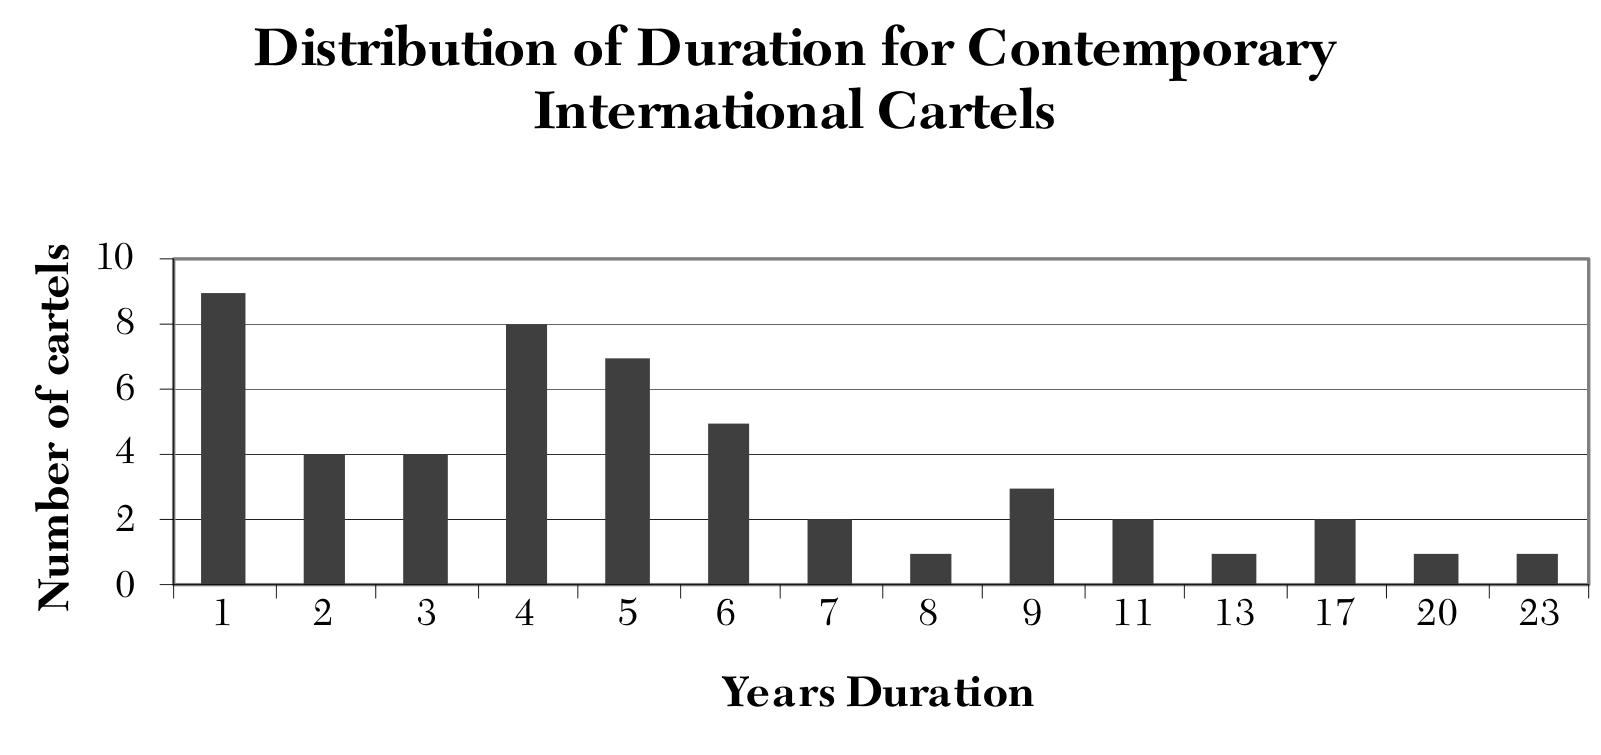
\includegraphics[width=0.78\textwidth]{figures/ch12/ls_fig1.png}
\caption{Distribution of the duration of contemporary international cartels. The horizontal axis lists only the
durations that occur, so it is not to scale. The underlying tabulation is from the authors' 2004 study (their source
note cites ``Levenstein and Suslow (2004b), table 1''). Source: \citet{LevensteinSuslow2006}, Figure~1.}
\label{fig:12-ls-duration}
\end{figure}

Case studies give longer durations (\cref{tab:12-ls-cases}). The nineteen industries contain fifty episodes of
cooperation, with a mean duration of 14 years, a median of 6 years and a standard deviation of 19.6 years
(p.~52). The median is close to the cross-section evidence, while the mean and the dispersion are much larger. The
authors attribute the difference partly to researchers' tendency to study industries with long or eventful cartel
histories. The DeBeers diamond cartel lasted 100 years before its first breakdown, while several cartels in the sample
barely got off the ground (p.~54). The Joint Executive Committee, the most studied cartel in modern economics
(\cref{sec:13-jec}), is the least stable in the sample. Its pools generally lasted two to five years and broke down
through entry or secret cheating (p.~56). Cooperation among southern U.S. railroads lasted three times as long on
average (footnote~40).

\begin{table}[htbp]
\centering
\caption{Cartel duration in selected case studies}\label{tab:12-ls-cases}
\footnotesize
\begin{tabular}{@{}l c r r r r@{}}
\toprule
Industry & First year & Mean duration & Episodes & Maximum & Minimum\\
\midrule
Beer (U.S.) & 1933 & 9 & 1 & 9 & 9\\
Beer (Sweden) & 1894 & 29 & 2 & 50 & 8\\
Bromine & 1885 & 6.25 & 4 & 10 & 3\\
Cement & 1922 & 40 & 1 & 40 & 40\\
Coal & 1893 & 20 & 1 & 20 & 20\\
Diamonds & 1870s & 60 & 2 & 100 & 20\\
Electrical equipment & 1950 & 8 & 1 & 8 & 8\\
Ocean shipping & 1870s & 51 & 3 & 54 & 50\\
Oil & 1871 & 2 & 3 & 3 & 1\\
Parcel post & 1851 & 28.5 & 2 & 40 & 17\\
Potash & 1877 & 9.4 & 8 & 20 & 1\\
Railroad (U.S. Midwest) & 1879 & 1.7 & 3 & 2 & 1\\
Railroad (U.S. South) & 1873 & 5 & 2 & 8 & 1\\
Railroad and oil & 1871 & 7 & 5 & 30 & $<1$\\
Rayon & 1932 & 8 & 1 & 8 & 8\\
Steel (Europe) & 1926 & 7.3 & 4 & 13 & 4\\
Steel (U.S.) & 1933 & 6 & 1 & 6 & 6\\
Sugar & 1887 & 6.75 & 4 & 10 & 2\\
Tea & 1929 & 3.5 & 2 & 6 & 1\\
\bottomrule
\end{tabular}

\smallskip
\begin{minipage}{0.86\textwidth}\footnotesize
Notes: Durations in years. ``First year'' is the first year of the first episode covered by the case studies.
``Episodes'' counts the distinct cartels that the studies date clearly. The episode-weighted mean of the column of
mean durations is 14 years, the figure reported in the text of the survey.
Source: \citet{LevensteinSuslow2006}, Table~2.
\end{minipage}
\end{table}

Is a typical life of five to six years long or short? The authors offer two benchmarks (pp.~56--57). The graphite
electrodes cartel, which lasted from mid-1992 to mid-1997, drew fines of more than 600 million U.S. dollars from U.S. and
European authorities. A cartel of average duration can thus inflict large damage. Firms themselves are not long-lived
either. Geroski reports that 61.5 percent of U.S. entrants exit within five years and 79.6 percent within ten, as
quoted by the authors. Cartels are less than perfectly stable. Yet they are about as durable as many other economic
organizations. The lesson is that cartels cannot be described simply as unstable. Some fail quickly, and others solve
the problems of coordination, cheating and entry for decades.

\subsection{Determinants of cartel duration}\label{sec:12-ls-determinants}

\citet[p.~57]{LevensteinSuslow2006} give two answers to the question of how cartels survive. Surviving cartels operate
in industries whose exogenous features make collusion easier. They also organize themselves to overcome
coordination, cheating and entry. Both are necessary and neither is sufficient.

\casehead{Number of firms and concentration}
The Bertrand constraint predicts that collusion is harder with more firms. The evidence is mixed. Most case-study
cartels and most contemporary international cartels operated in concentrated industries (p.~58). Yet the number of
participants in contemporary international cartels ranged from two to several hundred. Whenever there were more than
about half a dozen firms, an industry association or a government helped organize the agreement. In U.S. price-fixing
cases the mean number of conspirators is 7.25 in the sample of Hay and Kelley, which excludes four cases with 50 or more
conspirators. It is 16.7 in the sample of Fraas and Greer and 29.1 in that of Posner. Gallo et al. report a mean of 2.45 over all
2,689 Commerce Clearing House cases, not only horizontal conspiracies (Table~5). The medians are 7, 8, and
between 6 and 10. The shares of cartels with fewer than ten members are 79, 60 and 64 percent, and the average four-firm
concentration ratio in Hay and Kelley's sample is 77 percent (Table~5).

Effects on duration also conflict (Table~6, p.~61). Dick finds a statistically significant positive effect of the
number of firms on duration. Suslow finds a negative effect, which is not significant, and Hay and Kelley find no
significant pattern. Posner finds that 52 percent of the 79 cases with ten or fewer firms persisted six years or more,
against 64 percent of the 28 cases with more than ten firms. Hay and Kelley do find a positive association between
industry concentration and duration. Most of the conspiracies in their sample that lasted ten years or more were in
highly concentrated markets (Table~6, note~d, and p.~60). More consistently, duration rises with the share of the
market controlled by cartel members. The effect is positive and significant for Dick and Marquez, and positive but
not significant for Suslow. Marquez also finds a significant positive effect of cartel concentration, measured by a
Herfindahl index of the members' shares of cartel output. The authors offer three explanations for the weak link with concentration
(p.~58). Prosecutors may catch large cartels and association-run cartels more easily. Very concentrated industries may
collude tacitly and never appear in samples of explicit cartels. And concentration is endogenous, since collusion lets
more firms survive. Symeonidis finds a concave relation between the prevalence of collusion and concentration across
151 British industries (p.~60).

Trade associations are the organizational answer to large numbers. Posner reports that 44 percent of the cartels in
his sample used an industry association. Hay and Kelley, and Fraas and Greer, find associations in about a third of
U.S. conspiracies (p.~61). In the language of \cref{sec:12-cartels}, an association supplies the communication and
monitoring that large groups cannot achieve tacitly.

\casehead{Large customers}
\citet{Stigler1964} predicted that large buyers would tempt cartel members to cut prices secretly. The only explicit
econometric test, by Dick, finds that Webb-Pomerene export cartels selling to relatively larger buyers dissolved more
quickly (p.~61). Other evidence is less supportive. The citric acid cartel sold to firms such as Mars, Coca-Cola and
Procter \& Gamble, and the vitamins cartel to Kellogg, Quaker Oats and Tyson Foods (p.~62). These buyers do not seem to
have used their resources to break the cartels. The graphite electrodes investigation, started by a steel producer's
complaint, is the one exception the authors know. In five of the nineteen case studies, customers tried to break the
cartel (p.~62 and Table~7). In bromine and potash they tried to integrate backward, and in rayon they spread rumors of
cheating. In other cases customers helped stabilize a cartel and shared its rents. Customer size may destabilize a
cartel, while customer concentration may have the opposite effect.

\casehead{Demand}
Eckbo finds that cartels raised prices substantially only when demand was sufficiently inelastic with few short-run
substitutes (p.~64). The brewing industry, with a demand elasticity of $-10.3$, had an unsuccessful cartel,
with price wars in every year of the study (p.~64 and Table~8).

Demand instability matters more than the business cycle as such (Table~9). Dick finds that instability shortens
Webb-Pomerene cartels and that anticipated downturns end them, while unanticipated cycles have no significant
effect. Suslow finds significant negative effects of demand growth, of the business cycle and of unanticipated cycles.
Marquez finds a negative but insignificant effect of demand growth. Across case studies, macroeconomic fluctuations
seem to have had little relevance (p.~67 and Table~10). The international steel cartel is the only one reported to
have collapsed because of an observable demand shock. The authors read this as consistent with the Green-Porter and
Abreu literature, in which price wars follow unobserved rather than observed fluctuations. Their conclusion is that
unanticipated shocks and very rapid growth undermine cartels, while predictable cyclical fluctuations do not (p.~86).

This evidence must be mapped to the theory with care. The theories of \cref{sec:12-demand,sec:12-public} predict
changes in collusive prices or temporary price wars, not the end of a cartel. A Green-Porter reversion would appear as
a breakdown only if the researcher dates episodes by price wars. The finding that anticipated downturns end
Webb-Pomerene cartels fits the logic of \citet{HaltiwangerHarrington1991} and \citet{BagwellStaiger1997}, in which
collusion is hardest when future demand looks weak. It does not test whether the cartels died or merely punished.

\casehead{Organization and learning}
Successful cartels build organizations that monitor members, adjust the agreement to changing conditions, and settle
disputes (pp.~67--74). A joint sales agency is the strongest form, since it removes each firm's discretion over price.
Seven of the nineteen case-study industries used one: bromine, cement, diamonds, ocean shipping, oil, potash and
European steel. Most of these were among the more successful cartels (p.~69). Dick finds that a single sales agent
lowers the likelihood of cartel failure. Table~11 of the survey covers four U.S. cross-sections: Hay and Kelley,
Fraas and Greer, Posner, and Gallo et al. Trade associations were involved in 29, 36, 44 and 23 percent of their cases,
and market allocation in 35, 26, 26 and 27 percent. Suslow finds that self-imposed penalties significantly lengthen
cartel life (p.~71).

Hierarchies separate policy from day-to-day management. In the electrical equipment conspiracy of the 1950s, a working
group of sales managers devised the ``phases of the moon'' formula. It rotated the winning bidder for switchgear orders
every two weeks (pp.~72--73). In the citric acid cartel of 1991 to 1995, senior executives, nicknamed ``the
masters,'' set the broad agreement. Lower-level ``sherpas'' ran it. They shared monthly sales figures, and a firm that
sold more than its quota had to buy citric acid from a member below quota the next year (p.~73). This is the
quota-and-transfer scheme that \citet{HarringtonSkrzypacz2011} rationalize (\cref{thm:12-hs}).

Cartels learn. Dick and Suslow both find that prior cartel experience lengthens duration (Table~12). Within a single
episode, Dick finds that the hazard of dissolution rises with age. A cartel in its tenth year was 28 to 48 percent more
likely to dissolve than one in its fifth year. Several case-study cartels got off to a rocky start and later lasted for
long periods. Swedish brewers formed a cartel in 1894 with better control machinery than earlier attempts, and a
cartel formed in 1906 lasted fifty years (p.~74).

\casehead{Entry and exclusion}
Entry is a central threat. Dick finds that export associations formed where entry was slow, and Symeonidis that
collusion is more likely in capital-intensive industries (p.~74). Successful cartels create barriers to entry. Scott
Morton documents 47 cases of attempted entry against British shipping cartels. A typical price war against an entrant
lasted three months and cut prices by 50 percent on the routes the entrant served (p.~75). Nineteenth-century U.S. salt
producers, by contrast, saw each collusive arrangement collapse within a year or two because entry barriers were too
low (pp.~74--75).

\subsection{Why cartels break down}\label{sec:12-ls-breakdown-causes}

\Cref{tab:12-ls-breakdown} reproduces the causes of breakdown in international cross-sections. In Eckbo's first
sample, internal conflict or defection ended ten of twenty-three cartels, roughly 44 percent, and in his second sample
59 percent (p.~75). In Suslow's sample about a quarter ended because of internal conflict and cheating. Only World
War~II ended a larger share. Griffin finds that half of his cartels ended for political or external reasons
(p.~76). Entry or substitutes contributed to a third of his failures, and ``behavioral problems'' to another third. World War~II ended twelve of his cartels, and technological change ended four (rubber, zinc, sulfur and
nitrate). The category ``cheating and disagreement'' mixes monitoring failures with bargaining failures, which the
theory treats very differently.

\begin{table}[htbp]
\centering
\caption{Causes of cartel breakdown in international cross-section studies (percent of episodes)}\label{tab:12-ls-breakdown}
\footnotesize
\begin{tabular}{@{}l r r r r@{}}
\toprule
Cause of breakdown & Eckbo, sample 1 & Eckbo, sample 2 & Griffin$^{a}$ & Suslow\\
\midrule
Cheating and disagreement & 43.5 & 58.6 & 33.3 & 23.9\\
External shock & 30.4 & & 50.0$^{c}$ & 42.3\\
Entry and substitution$^{b}$ & 26.1 & 41.4 & 33.3 & 15.5\\
\quad Entry & 13.0$^{b}$ & & 25.9 & 15.5\\
\quad Substitution & 8.7$^{b}$ & & 9.3 & \\
Technological change & & & 9.3 & \\
Antitrust indictment & & & & 18.3\\
\midrule
Total number of episodes & 23 & 29 & 54 & 71\\
\bottomrule
\end{tabular}

\smallskip
\begin{minipage}{0.92\textwidth}\footnotesize
Notes: Blank cells are not reported. (a) Based on Griffin's discussion and on his Table~4. Griffin lists more than one
cause for several cartels, so his column sums to more than 100. The survey's text names four cartels ended by
technological change (4 of 54, or 7.4 percent), while the table reports 9.3 percent. Its footnote~90 notes that
Griffin's own text and table differ. We reproduce both figures as printed. (b) Entry and substitution do not always add to the
total, because Eckbo leaves one episode unclassified and Griffin counts two cartels under both. Of Eckbo's six
episodes in this category, three ended through entry, two through substitution and one is unclassified. (c) Griffin
groups wars, antitrust and other government actions, and cartel reorganizations. Some reorganizations may be
bargaining problems, so the entry overstates external shocks as classified here.
Source: \citet{LevensteinSuslow2006}, Table~13.
\end{minipage}
\end{table}

Case studies separate these causes better (Table~14 of the survey, p.~77). Entry was the primary cause of
disruption in just over a third of the episodes. World Wars~I and~II ended about 15 percent and legal action a little
over 10 percent. Only three episodes, fewer than 10 percent, ended because of cheating (p.~78). Bargaining problems
affected virtually every cartel and ended about a quarter of the episodes. Many case-study authors report that
cheating was simply not a problem.

Successful cartels avoided costly punishments. The Sugar Institute ``served as a court in which an accused firm might
prove its innocence'' \citep[p.~389]{GenesoveMullin2001}, as quoted by \citet[p.~78]{LevensteinSuslow2006}. Outside
the South, deviations ``were either ignored or matched'' rather than met by reversion to competition
\citep[pp.~390--391]{GenesoveMullin2001} (see \cref{sec:13-sugar-institute}). In steel in the 1930s, unexpected
declines in demand led to ``shallow episodes of increased competition,'' in Baker's words, rather than severe price
wars. In bromine, violations were answered with negotiated side payments rather than price wars
(\citealp{Levenstein1997}, \cref{sec:13-bromine}). The authors conclude that Cournot reversion is an inefficient way to
sustain collusion, as the cartel members themselves repeatedly discovered (p.~78).

\citet[p.~79]{LevensteinSuslow2006} draw three lessons. First, the outbreak of a price war, as opposed to its threat,
is rarely a sign of cartel success. Second, the most successful cartels develop alternative punishments and threats
that sustain collusion at lower cost. Third, cartels break down sometimes because of cheating, but more often because
of entry, exogenous shocks and dynamic changes within the industry.

\subsection{Effects on prices}\label{sec:12-ls-prices}

Rigorous counterfactual estimates of cartel overcharges are rare (p.~45). The available evidence nonetheless shows that
many cartels raised prices substantially (pp.~80--81). Eckbo finds that nineteen of fifty-one cartels raised price 200
percent above the unit cost of production and distribution. Griffin finds an average markup of 45 percent over marginal
cost. His most successful cartel, rubber from 1923 to 1928, had a markup of 400 percent, while his least successful,
wheat from 1933 to 1934, priced below cost. For contemporary international cartels, reported price increases, mostly
from the trade press, range from 10 to 100 percent. Graphite electrode prices rose more than 50 percent in the United
States from 1992 to 1997. In Canada, where two firms held more than 90 percent of the market, they rose more than 90
percent. Some evidence points the other way. Fölster and Peltzman find that legal Swedish cartels did not raise prices,
although a re-examination of the same data by Ciarreta finds that they did. In 25 price-fixing cases from 1973 to 1984,
Sproul finds that prices four years after indictment were slightly higher, by 7 percent.

Case studies seldom measure success against a counterfactual (p.~81 and Table~15). Hausman finds that the regulations
of the ``Limitation of the Vend,'' a coal cartel in northeast England from 1770 to 1845, raised the equilibrium price
by about 6 to 8 percent. Bromine prices came close to the joint-profit-maximizing level in some periods and barely
exceeded the Cournot level in others. Ocean shipping was close to the joint-profit level. The German steel cartel
priced below the joint-profit level but one-third above the world price. The cement cartel priced 10 percent above
the world price. Diamond prices nearly doubled after the cartel formed, and tea prices rose 80 percent
in 1933 after the cartel was reestablished. The U.S. beer cartel of the 1930s may even have priced above the monopoly
level, under political pressure to keep alcohol expensive. Yet it had price wars in each of the three years it tried
to collude. Success must be judged over the whole life of a cartel, not only during its collusive periods (p.~81). The
methods for estimating overcharges and damages are developed in \cref{sec:13-damages}.

\subsection{What the evidence says about the theory}\label{sec:12-ls-theory}

The survey speaks to each part of the theory in this chapter.
\begin{enumerate}[label=(\arabic*)]
\item \emph{Structure.} The perfect-monitoring theory of \cref{sec:12-perfect} predicts that collusion is easier with
fewer firms. Concentration helps, but organization can substitute for it, and concentration is itself shaped by
collusion.
\item \emph{Demand.} Unanticipated shocks and rapid growth undermine cartels, while predictable cycles do not. This
pattern matches the role of unobserved shocks in \citet{GreenPorter1984}. The evidence on anticipated downturns fits
the persistent-demand models of \cref{sec:12-demand}. Cross-section data on cartel deaths cannot test the
within-cartel price dynamics these models predict. That requires the time-series studies of \cref{sec:13-jec}.
\item \emph{Price wars.} Many observed price wars are bargaining wars or breakdowns. Successful cartels prefer
monitoring, courts and side payments to Green-Porter reversions. This supports the shift of the theory toward
communication and transfers (\cref{sec:12-cartels}) and toward tolerated cheating (\cref{rem:12-bm},
\cref{sec:13-imperfect}).
\item \emph{Organization.} Joint sales agencies, reporting systems, penalties and hierarchies lengthen cartel life.
Theory treats them as devices that make information public or transfers possible, as in
\citet{HarringtonSkrzypacz2011}.
\item \emph{Entry.} Entry is the most common cause of breakdown in the case studies, yet most repeated-game models
hold the set of firms fixed. This is the largest gap between the theory and the evidence.
\item \emph{Enforcement.} Antitrust action ended 18.3 percent of Suslow's interwar international cartels and a little
over 10 percent of case-study episodes. Enforcement also selects which cartels we observe, as \cref{sec:12-enforcement}
and \cref{sec:13-institutions} discuss.
\end{enumerate}

The survey has limits. It aggregates studies with different definitions of a cartel, of an episode and of a cause of
breakdown. Most of its quantitative statements are counts and percentages, not estimates with standard errors. Selection
is unavoidable and of unknown sign. The cross-section regressions it summarizes use duration as the dependent variable,
which is a noisy measure of success, and they rarely control for the endogeneity of structure and organization. Its
contribution is to replace the presumption that cartels are inherently unstable with a set of facts. Cartels often
last for years. They end more often through entry, shocks and bargaining than through secret cheating. The successful
ones invest in organization.

\section{Synthesis: What the Theory Predicts and How to Test It}\label{sec:12-synthesis}

\Cref{tab:12-models} collects the models of this chapter. Each row states what firms observe, why collusion is hard,
what the most collusive equilibrium looks like, whether price wars occur on the equilibrium path, and what the model
predicts for prices. The last column points to the section of \cref{ch:collusion-evidence} where the prediction meets
data.

The table carries five lessons for empirical work.

The first lesson is that theory delivers a set of sustainable outcomes and leaves the choice among them open. The
folk theorem and
\cref{cor:12-bertrand-any-price} imply that a wide range of prices can be sustained in the same environment. Empirical
work that tests ``collusion'' must therefore commit to a specific model of how the cartel operates. The common
selection, the most collusive equilibrium, is a convention.

The second lesson is that conduct varies over time. In Rotemberg and Saloner, Haltiwanger and Harrington, and Bagwell
and Staiger, collusive margins move with current and expected demand. In Green and Porter, conduct switches between
regimes. A constant conduct parameter then averages over states, which is the critique of \citet{Corts1999} discussed
in \cref{ch:conduct}. Estimation must allow for regimes or for state-dependent conduct, as the methods of
\cref{sec:13-implications} do.

The third lesson is that a price war is an ambiguous signal. In \citet{GreenPorter1984} it is part of a working
cartel. In \citet{Stigler1964} and in the bargaining wars documented by \citet{LevensteinSuslow2006}, it marks a
failing one. The timing of wars relative to demand helps discriminate. Wars after unexpected drops in demand point to
Green and Porter. Low prices in booms point to Rotemberg and Saloner. Wars around entry or renegotiation point to
bargaining. \Citet{Ellison1994} uses exactly this logic to test Green and Porter against Rotemberg and Saloner in the
railroad cartel of \citet{Porter1983} (\cref{sec:13-ellison}).

The fourth lesson is that communication and transfers are observable in prosecuted cartels, and they matter most when
information is private. The anatomy of the lysine and citric acid cartels, with quotas, sales reports and buy-backs, is
predicted by \citet{HarringtonSkrzypacz2011}. The identical bidding of many rings is predicted by
\citet{AtheyBagwellSanchirico2004}, and their take-turns scheme is a model of bid rotation. Evidence on the internal organization of cartels can thus discriminate among
models in a way that price data alone cannot.

The fifth lesson is that detection needs a competitive benchmark and a theory of the specific cartel. Overcharges are
measured against a but-for price. Tests of bid rigging compare suspected firms with a model of noncooperative bidding.
Enforcement determines which cartels enter the data, so every finding is conditional on how the cartels were found.

\begin{landscape}
\begin{table}[p]
\centering
\caption{Models of collusion and their testable implications}\label{tab:12-models}
\scriptsize
\renewcommand{\arraystretch}{1.1}
\begin{tabularx}{\linewidth}{@{}>{\raggedright\arraybackslash}p{2.5cm}
>{\raggedright\arraybackslash}X >{\raggedright\arraybackslash}X >{\raggedright\arraybackslash}X
>{\raggedright\arraybackslash}p{2.7cm} >{\raggedright\arraybackslash}X
>{\raggedright\arraybackslash}p{2.1cm}@{}}
\toprule
Model & What firms observe & Source of the incentive problem & Most collusive equilibrium and price pattern & Price
wars on the path? & Testable implication & Tested in\\
\midrule
Perfect monitoring, Bertrand and Cournot (\cref{sec:12-perfect}) & All past prices or outputs & One-period gain from
undercutting against the loss of future collusion & Stationary price, monopoly if $\delta \ge \underline\delta(N)$.
Any price in $[c, p^m]$ can be sustained & No & Collusion is easier with fewer, more symmetric firms, frequent
interaction and transparency & \cref{sec:13-information}, \cref{ch:mergers}\\
Rotemberg and Saloner (\cref{sec:12-demand}) & Current demand (\iid) and past prices & Gain from cheating rises with
current demand, future loss is constant & Monopoly price in low states, capped profit in high states. Countercyclical
margins & No, unless prices are restricted to collude or compete & Margins fall when current demand is high relative
to expected demand & \cref{sec:13-jec}, \cref{sec:13-gasoline}\\
Haltiwanger and Harrington (\cref{sec:12-demand}) & A known demand cycle & Future loss is small when demand is about
to fall & Prices lowest when demand is about to fall, and at the peak only for impatient firms & No & Margins rise with expected future demand &
\cref{sec:13-gasoline}\\
Bagwell and Staiger (\cref{sec:12-demand}) & Current growth phase (Markov) & Gain and loss both move with the phase &
Procyclical prices if growth rates are positively correlated, countercyclical if negatively & No & Cyclicality
depends on the persistence and expected durations of phases & \cref{sec:13-predictions}\\
Green and Porter (\cref{sec:12-public}) & Market price only & A low price may reflect cheating or low demand &
Trigger price, reversion of finite length. Regime switching & Yes, after unexpectedly low prices & Wars follow
negative demand shocks and have finite length & \cref{sec:13-jec}\\
Athey, Bagwell and Sanchirico (\cref{sec:12-private-costs}) & Public prices, private \iid\ costs & Low-cost firms want
more market share & Patient firms: one rigid price, equal shares. Impatient firms: an escape clause & No (inelastic
demand) & Rigid, identical prices that ignore firm-specific costs & \cref{sec:13-detection}, \cref{sec:13-legal}\\
Harrington and Skrzypacz (\cref{sec:12-cartels}) & Own sales and public reports & Secret price cuts, unverifiable
sales reports & Quotas, sales reports and per-unit transfers. Breakdown after low total reports & Yes, rare
breakdowns & Quota schemes with buy-backs, breakdowns after low sales & \cref{sec:13-imperfect}\\
Bernheim and Madsen (\cref{rem:12-bm}) & All quotes, with costly quoting and home cost advantages & Raiding the
rival's home market & Price floor below the home monopoly price. Dispersed prices & No. Raids above the floor are
tolerated & Business stolen at higher prices is less likely to be punished & \cref{sec:13-imperfect}\\
Chen and Rey (\cref{sec:12-chenrey}) & Own conduct, random detection, leniency & Cheat and report, or collude and
report & Normal collusion if the stake exceeds the deterrence threshold & No (binary conduct) & Excessive leniency
induces systematic self-reporting & \cref{sec:13-enforcement}, \cref{sec:13-asker}\\
\bottomrule
\end{tabularx}

\smallskip
\begin{minipage}{\linewidth}\scriptsize
Notes: Our synthesis of the models in this chapter. \citet{BernheimMadsen2017} is developed in
\cref{sec:13-imperfect}. Price wars on the path refer to the most collusive equilibrium of each model.
\end{minipage}
\end{table}
\end{landscape}

\Cref{ch:collusion-evidence} takes these lessons to data. It begins with the econometrics of regime switching
(\cref{sec:13-implications}) and the Joint Executive Committee (\cref{sec:13-jec}), where the Green-Porter and
Rotemberg-Saloner predictions are tested. It continues with the rules and communication of legal cartels, information
exchange, retail gasoline, tolerated cheating, the internal organization of a bidding ring, and the statistical
detection of bid rigging. It ends with enforcement and the measurement of damages (\cref{sec:13-enforcement}).
